\documentclass[a4paper,10pt]{book}

\usepackage[utf8]{inputenc}
\usepackage[english]{babel}
\usepackage{euscript}
\usepackage{epigraph}

\usepackage{graphicx}
\usepackage{amsmath}
\usepackage{amssymb}
\usepackage{amsthm}
\usepackage{fancyhdr}


\usepackage{pictexwd,dcpic}

\usepackage{wrapfig}


%-------------- Margins
\setlength{\oddsidemargin}{20pt}
\setlength{\evensidemargin}{20pt}
\setlength{\marginparwidth}{-20pt}
\setlength{\textwidth}{400pt}
\setlength{\topmargin}{-15pt}
\setlength{\textheight}{640pt}

%--------------- Quotient
\def\quotient#1#2{%
	\raise1ex\hbox{$#1$}\Big/\lower1ex\hbox{$#2$}%
}

% ----------------- Argmin
\newcommand{\argmin}{\operatornamewithlimits{argmin}}

%------------ Theorems and maths --------
\theoremstyle{definition}
\newtheorem{definition}{Definition}[section]
%\theoremstyle{plain}
\newtheorem{example}{Example}[section]
\newtheorem{lemma}{Lemma}[section]
\newtheorem{observation}{Observation}[section]
\newtheorem{theorem}{Theorem}[section]
\newtheorem{prop}{Property}[section]
\newtheorem{corollary}[theorem]{Corollary}%[section]
\newtheorem{algorithm}{Algorithm}

%---------- Proof
%\newenvironment{proof}{\par\addvspace\topsep\noindent
%{\bf Proof:} \ignorespaces }{\qed}
%\newcommand{\qed}{\hspace*{\fill}$\Box$\ifmmode\else\par\addvspace\topsep\fi}


%------------ Norm
\newcommand{\euclideanMetric}[1]{\vert\lvert #1 \rvert\vert}
\newcommand{\supMetric}[1]{\vert\lvert #1 \rvert\vert_{sup} }

\newcommand{\quotes}[1]{\text{ \lq\lq  #1\rq\rq\phantom{z}}}


\RequirePackage{hyperref}
\hypersetup{ hidelinks=true}

\begin{document}


%%%%%%%%%%%%%%%%%%%%%%%%%%%%%%%%%%%%%%%%%%%%%%
%%%%%%%%%%%%%%%%INIZIO FRONTESPIZIO
\begin{titlepage}
%
\pagestyle{empty}
\begingroup
% INTESTAZIONE
\vspace*{-7\topskip}

\vspace{-0.95 cm}

\begin{figure}[!h]
	%centrare
	%\begin{flushright}
	%\centering
		\hspace{-2.5cm} % 5mm away from the left + offset
		\resizebox{19.8 cm}{5.5 cm}{
			
\includegraphics{figures/UCL-logo3.pdf}
			} %1.5 2.5
	%\end{flushright}
\end{figure}
\vspace{1cm}

\begin{center}
	{\LARGE{Sebastiano Ferraris}\par}
\end{center}
\vspace{1.8cm}
\begin{center}
        {\huge\bf \baselineskip=0.95em plus 1pt \expandafter{
        The Log-composition of Stationary Velocity Fields in Diffeomorphic Image Registration
        \par}}
\end{center}



\vspace{2.7cm}

\begin{center}
	\LARGE{\rm\expandafter{University College London}}\par
	\expandafter{\Large{Medical Physiscs and Biomedical Engineering}\par}
\end{center}

\vspace{1cm}

\begin{center}
	A dissertation submitted in partial fulfillment 
	\\
	of the requirements for the degree of
	\\ 
	{\bf Master of Research}	
\end{center}

\vspace{0.2cm}
\begin{center}
	\today
\end{center}

\vspace{2.0cm}
%%\vspace{0.5cm}
%\begin{center}
%	{\LARGE{Tesi di Laurea Magistrale}\par}
%\end{center}

\begin{center}
\begin{tabular}{l p{1.5cm} l p{1.5cm} l}
	Supervisor&   & Co-Supervisor & &  Clinical Supervisor \\
	\textbf{Tom Vercauteren} &  & \textbf{Marc Modat}& & \textbf{Jan Deprest}  \\
\end{tabular}
\end{center}

%CHIUSURA
\par
\vfill\par 

\endgroup


\end{titlepage}

%%%%%%%%%%%%%%%%% PAGE JUMPERS:
%%%%%%%%%%%%%%%%%%%%%%%%%%%%%%%%%%%%%%%%%%%%

% \qquad
%  \thispagestyle{empty}
% \newpage
% \qquad
%  \thispagestyle{empty}
% \newpage

%\qquad
%  \pagestyle{empty}
% \newpage

 
%%%%%%%%%%%%  SOMMARIO


\qquad
\pagestyle{empty}
\newpage


% % % % % % % % % % % % % % % % % % % % % % % % % % % % % % % % % % % % % %
% % SUB SECTION
% % % % % % % % % % % % % % % % % % % % % % % % % % % % % % % % % % % % % %
\section*{Abstract}

Medical imaging employs techniques and tools belonging to several branches of mathematics and physics that, when applied to morphometric and statistical study of biological shape variability, are collected under the name of \emph{computational anatomy}. 
One of its critical tool, image registration, is widely used in both academical studies and applications, and continuously challenges researchers to enhance accuracy, improve reliability and reduce the time of the computations. The use of diffeomorphisms in image registration and the concomitant introduction of the log-euclidean framework to compute statistics, provide an interesting options to model the organs' deformations and to quantify the variations of anatomies.
One of the challenge of this setting are the numerical computation of the Lie exponential of stationary velocity fields (SVF), the Lie logarithm of the corresponding transformation and their combinations as they appear in the BCH formula: concept at the core of the underpinning theory of the \emph{log-demons} algorithm.\\
The necessity of finding fast numerical computation techniques of the BCH formula gave birth to the concept of log-composition presented in this thesis within some strategies for its computation.


% % % % % % % % % % % % % % % % % % % % % % % % % % % % % % % % % % % % % %
% % SUB SECTION
% % % % % % % % % % % % % % % % % % % % % % % % % % % % % % % % % % % % % %
\section*{Thesis' Organization}
%Four chapters, all alike in dignity are presented in this fair thesis: \\
\begin{enumerate}
	\item[{\bf Chapter \ref{ch:introduction}}] The first chapter is devoted to the introduction of diffeomorphic image registration and the main recent advancements. Here are introduced advantages and disadvantages of using diffeomorphisms as well as some of the milestone frameworks that led to, or are directly affected by the log-composition.
	
	\item[{\bf Chapter \ref{ch:tools}}] The second one is the chapter of mathematical elements and tools. We introduce main definitions and results from differential geometry directly involved in the proposed numerical methods, as Lie logarithm, Lie exponential, connections and parallel transport.
	The concept of log-composition, around which the research gravitates, is defined as consequence of the need of generalize the BCH formula, and we propose the first steps for its computation. 
	
	\item[{\bf Chapter \ref{ch:spatial_transformations}:}] In this section we introduce two sets of transformations on which the numerical methods will be tested and compared. The first set consists in the finite dimensional group of rigid body transformation of the plane: here logarithms and exponentials possess a closed form, therefore a ground truth to compare the methods is available.
	The second set of transformation on which numerical methods are applied are the set of diffeomorphisms corresponding to the infinite dimensional stationary velocity fields in the tangent space. For this second case no closed form are available, but comparing the exponential it is still possible to find a ground truth respect to which compare results.
	
	\item[{\bf Chapter \ref{ch:log_computations}:}] The algorithm to compute the logarithm (here called \emph{log-algorithm}) presented in \cite{Bossa2007} is grounded on the BCH formula and can be cleanly reformulated using the log-composition. Each numerical method to compute the log-composition become naturally available to challenge its performance.
  
	\item[{\bf Chapter \ref{ch:results}:}] Here we are at the experimental results. The log-composition applied to rigid and diffeomorphic registration is applied to synthetic data and clinical images. \\
	
	
\end{enumerate}









  % abstract and organization of chapter

%%%%%%%%%%%%  INDICE

\pagestyle{plain}  \pagenumbering{Roman}
\tableofcontents



%%%%%%%%%%%%%%%%%%%%%%%%%%%%%%%%%%%%%%%%%%%%%%%%
%%%%%%%%%%%%%%%%%%%%%% CAPITOLI     %%%%%%%%%%%%%%%%%%%%
%%%%%%%%%%%%%%%%%%%%%%%%%%%%%%%%%%%%%%%%%%%%%%%%

\newpage
\pagestyle{fancy} \pagenumbering{arabic}


\fancyhead{} % clear all header fields

\fancyhead[LE]{\slshape \rightmark}

\fancyhead[RO]{\slshape \leftmark}
\fancyfoot[C]{\thepage}
\renewcommand{\headrulewidth}{0.4pt}
%\renewcommand{\footrulewidth}{0.4pt}


%\fancyhead[RO,LE]{\bfseries The performance of new graduates}
%\fancyfoot{} % clear all footer fields
%\fancyhead[LE,RO]{\thepage}
%\fancyhead[LO]{\thesection}
%\fancyhead[RE]{\thechapter}
%%\fancyfoot[CO,RE]{To: Dean A. Smith}
%\renewcommand{\headrulewidth}{0.4pt}
%%\renewcommand{\footrulewidth}{0.4pt}

\chapter{Introduction: Diffeomorphisms in Medical Imaging Registration}\label{ch:introduction}


\begin{flushright}
		\emph{The series is divergent, therefore we may be able \\ to do something with it.}\\
			- Oliver Heaviside
\end{flushright}

\vspace{0.6cm}


The log-composition is an inner binary operation defined on the tangent space of a group of transformations, that reflects the properties of the group's composition. It arises in medical image registration, when diffeomorphisms are utilized to model the transformation of anatomies between images. Before proposing its formal definition within its context, is necessarily to introduce the diffeomorphic demons algorithm, and so to spend some worlds about the medical image registration problem in general. 

\section{Toward an ill-posed Problem}
Medical image registration is a set of tools and techniques aided to solve the problem of determining correspondences between two or more images acquired from patients scans. It is a challenging task that has seen the application of a growing number of mathematical theories contributing to its solution.

Involved difficulties are a consequence of the fact that dealing with image registration problem means dealing with an ill-posed problem. Transformations between anatomies are not unique, and the impossibility to recover spatial or temporal evolution of an anatomical transformation from temporally isolated images, makes any validation a difficult, if not an impossible task. 
In addition each situation inevitably brings some prior knowledge within the initial data, that may imply some modifications in the problems' setting and may imply some additional constraints. This, of course, impact dramatically the range of possible choices in searching for a solution and in the consequent results. 

Certainly it is the practical situation that provides the hint in choosing the optimal constraints, but it almost never provides enough information to reduce the large amount of options involved. A wide range of variants in methodologies and approaches to solve the registration problem has been thus proposed in the last decades: a quick glance to Google scholar reveals about $1200000$ papers in \emph{medical image registration} (55\% of the whole \emph{image registration} resources). 

\subsection{Some Examples of Medical Image Registration}
One of the most studied application of image registration is in the domain of brain imaging: there this tool can be used to examine differences between subjects and distinguish their biological features - cross-sectional studies - or to compare different acquisition of the same subject after a fixed period of time or before and after a surgical operation - longitudinal studies -. 

In both cross-sectional and longitudinal studies an accurate comparison between images and the parameters of the transformation involved may result in a quantification of anatomical variability and in a better understanding of the patients' features. 
%
For example, brain atrophy is considered a biomarker to diagnose Alzheimer disease and to analyze its evolution; most of the algorithms and techniques involved in the atrophy measurement require longitudinal or cross-sectional scans to be aligned, and so are directly affected by the solution of the registration algorithm \cite{prados2015measuring}, \cite{fox1997brain}, \cite{gauthier2012prevention}. 

Also when dealing with motion correction, if a sequence of images is affected by the motion of cardiac pulses or respiratory cycles, registration algorithms are often used for the realignment. 
For example, in lungs radiotherapy, the correspondence between the lungs' deformation and the respiratory signal defines a model to direct the X-ray or electrons beam on the cancer, avoiding as much as possible the sane tissue. Lungs deformation is obtained using a registration algorithms that provides the direction of the motion of each voxel in each phase of breathing \cite{mcclelland}, \cite{mcclelland2011inter}.

Another application of image registration is the operation of peacing together several pictures with partially coincident regions, aided to obtain a bigger image of the whole scene. This procedure, called \emph{mosaicing}, exploit registration algorithms to aligns images using information obtained form the overlapping regions \cite{vercauteren2006robust}, \cite{szeliski1994image}.

The next section moves toward some details of one iterative framework most commonly utilized by image registration algorithms.

% % % % % % % % % % % % % % % % % % % % % % % % % % % % % % % % % % % % % %
% % SUBSECTION
% % % % % % % % % % % % % % % % % % % % % % % % % % % % % % % % % % % % % %

\subsection{Image Registration Problem}\label{se:registration_framework}

A \emph{$d$-dimensional image} is a continuous function from a subset $\Omega$ of the coordinate space $\mathbb{R}^{d}$ (having in mind particular cases $d=2,3$) to the set of real numbers $\mathbb{R}$. Given two of them, $F : \Omega_{F}  \rightarrow\mathbb{R} $ and $M : \Omega_{M}  \rightarrow\mathbb{R} $, called respectively \emph{fixed image} and \emph{moving image}, the \emph{image registration problem} consists in finding the transformation function
\begin{align*}
\varphi :\mathbb{R}^{d} \supseteq \Omega_{F} & \longrightarrow \Omega_{M}\subseteq \mathbb{R}^{d}   \\
\mathbf{x} &\longmapsto \varphi (\mathbf{x}) 
\end{align*}
such that for each point $\mathbf{x}\in \Omega_{F} $ the element $M(\varphi (\mathbf{x}))$ and $F(\mathbf{x})$ are as closed as possible according to a chosen measure of similarity. Other than obtaining $\varphi$, also the investigation of its features and parameters are a part of the problem.

The definition of image registration problem proposed here can be represented by the following diagram, where $\varphi$ is the solution that makes $f$ the identity function:

\[
\begindc{\commdiag}[40]
\obj(-30,30)[Or]{$\Omega_{F}$}
\obj(0,30)[Ot]{$\Omega_{M}$}
\obj(-30,10)[Rref]{$\mathbb{R}$}
\obj(0,10)[Rtarg]{$\mathbb{R}$}

\mor{Or}{Ot}{$\varphi$}
\mor{Or}{Rref}{$F$}
\mor{Ot}{Rtarg}{$M$}
\mor{Rref}{Rtarg}{f}[1,1]

\enddc
\]
% fine diagramma
\noindent
The composition of the moving image after the transformation, $M\circ\varphi $, is called \emph{warped image}, and
if $\Omega_{F} \neq \Omega_{M}$, it is always possible to apply an homeomorphism to transform them into a common domain $\Omega$, called  \emph{background space}, on which both of the images are defined. 

This setting leaves two main degrees of freedom in searching for a solution: the transformation's domain to which $\varphi$ belongs (also called \emph{deformation model}), and the metric to measure the similarity between images. 
Once these are chosen, they are the main constituent of the \emph{image registration framework}: 
an iterative process that provides at each step a new function $\varphi$ that approach one of the possible solution to the registration problem.

% % % % % % % % % % % % % % % % % % % % % % % % % % % % % % % % % % % % % %
% % SUB SECTION
% % % % % % % % % % % % % % % % % % % % % % % % % % % % % % % % % % % % % %
\subsection{Iterative Registration Framework}

The definition of registration problem and the iterative framework described above, raise several issues. For example there are no reasons to believe that the correspondence that models the deformation between images is unique. In addition the condition $M(\varphi (\mathbf{x})) = F(\mathbf{x})$ for each point $\mathbf{x}\in \Omega_{F} $ can be satisfied by functions that do not represents any reasonable biological transformation between anatomies.

One way to deal with these issue is to add some constraints on the transformation $\varphi$, such that it is bound to model realistic changes that can occur in biological tissues. The kind and quality of the constraints are one of the features that distinguish one registration algorithm to the other, and they can be mathematically expressed by the definition of a deformation model and an \emph{energy function} (or objective function). This last measures the similarity $\text{Sim}$ between the fixed image and the warped image plus an additional regularization term $\text{Reg}$ that 
add further constraints on the transformation penalizing its measured irregularities:
\begin{align}\label{eq:general_cost_function}
\mathcal{E}(F, M, \varphi) = \text{Sim}(F,M,\varphi) + \text{Reg}(\varphi) 
\end{align}
An optimization algorithm is then utilized to minimize the equation \ref{eq:general_cost_function} and to provide the sought transformation, bonded to a chosen domain.

Finally, since the images are modeled by continuous functions, but are represented as discrete structure, a resampling technique has to be chosen among several options (see for example\cite{gonzalezdigital}). 
Computational complexity of resampling is $\mathcal{O}(1)$ and its choice has a relatively small impact on the image registration algorithm, nevertheless it implies another range of possibility in the definition of the registration framework.

According to what has been said we can represent the iterative registration framework as a device with $5$ parameters, each with its range:
\begin{align*}
\{  \varphi \} &\in \{ \text{Transformations}\}\\
\text{Sim} &\in \{ \text{Similarity measures}\}\\
\text{Reg} &\in \{ \text{Regularization Terms}\}\\
\text{Opt} &\in \{ \text{Optimization techniques}\}\\
\text{Res} &\in \{ \text{Resampling techniques}\}\\
\end{align*}
They provide the constraints required by the algorithm to solve the image registration problem, according to the specific constraints provided by the situation. 
\begin{figure}[!ht]
	\centering
	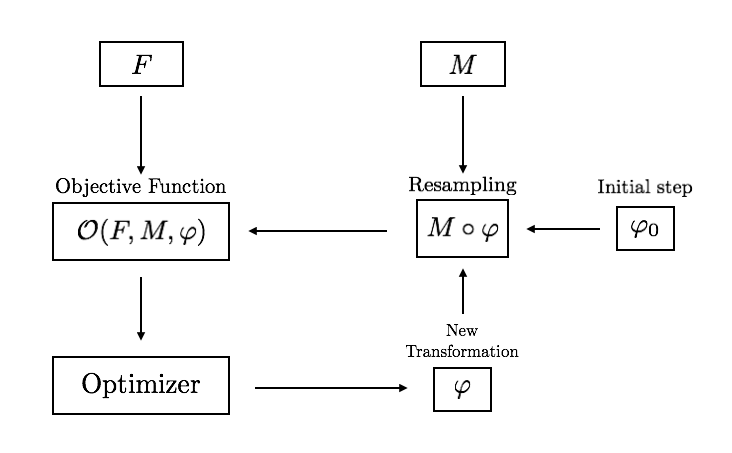
\includegraphics[scale=0.235]{figures/iterative_algorithm.png}
	\caption{Flowchart of the image registration framework.}
	\label{fig:iterative_algorithm_scheme}
\end{figure}
The flowchart of the framework is show in figure \ref{fig:iterative_algorithm_scheme}. Given a fixed and a moving image and an initial transformation $\varphi_0$, the warped image $M\circ\varphi_{0}$ is computed, and the 
energy function \ref{eq:general_cost_function} is optimized at each step by the algorithm. The resulting new transformation $\varphi$ takes the place of $\varphi_0$ for the subsequent steps.

Many of the available registration algorithms follow this scheme, and the specific choice of the $5$ parameters involved provides a preliminary classification of the algorithm.
For further details see for example the recent surveys \cite{Sotiras:survey:13} and the less recent one \cite{zitova2003image}. 

% % % % % % % % % % % % % % % % % % % % % % % % % % % % % % % % % % % % % %
% % SECTION
% % % % % % % % % % % % % % % % % % % % % % % % % % % % % % % % % % % % % %
\section{Diffeomorphisms in Medical Imaging Registration}

In the one presented above, as well as in any other  image registration algorithm framework, one of the most relevant feature is the choice of the family to whom the transformation belongs. This is as an important constraint that change according to the aim of the registration and to the nature of the objects represented by the images. 

If the algorithm is meant to model transformations that preserve distances, orientations and angles, then the set of transformations can be bonded to the group of rigid rotations and translations $SE(3)$. The consequent registration algorithm, called \emph{rigid-registration algorithm}, will be suitable for example to compensate the motion in a rapid sequence of scans, or to investigate small differences that occurs in longitudinal scans.

If the algorithm is meant to model transformations that only preserves topology, then the transformations must allow more freedom than the one chosen for the rigid case. It is in this context that the mathematical objects of diffeomorphisms are taken into account. These are defined as bijective differentiable maps with differentiable inverse, and are particularly well suited to model non-rigid deformations between images (for a more  general introduction see for example \cite{lee2012introduction}, \cite{arnold2006ordinary}). Consequent algorithms are called \emph{diffeomorphic registration algorithms}.

These algorithms, thanks to the property of invertibility and topology-preserving of the transformations involved, appears to be a natural choice to model organs' deformations and in many cases are the ideal candidate for the set of transformation in the registration framework. This is due to the fact that in longitudinal studies, anatomies are involved in a smooth process of modification over time that do not presume breaking of topology. Also in most of the cross-sectional studies variations in the topology of the same organ in different patients are not expected. 

It is importance to notice that, when implemented in image registration algorithms, diffeomorphisms do not have only radically different results than the rigid body transformations: they also possess a radically different mathematical structure.

% % % % % % % % % % % % % % % % % % % % % % % % % % % % % % % % % % % % % %
% %  SUBSECTION
% % % % % % % % % % % % % % % % % % % % % % % % % % % % % % % % % % % % % %
\subsection{Utility and Liability of Diffeomorphisms}\label{se:diffe_util_and_liab}

On the algebraic side, the set of diffeomorphisms appears particularly interesting for their group structure and within their differentiable nature (see for example \cite{michor1980manifolds} and \cite{lempert1997problem}). They have also an infinite-dimensional structure of vector space, and their mathematical formalization as Lie group (so as differentiable manifold within a group structure, see \cite{warner}, \cite{lee2012introduction}) is an open field of research whose development has not yet reach a definitive formalization.

Attempt to provide some handles to the group of diffeomorphisms for easy manipulation was done for the first time in 1966 by Vladimir Arnold \cite{arnold1966geometrie} (see also the equivalent \cite{arnold1998topological}, more readable for non-French speakers). To solve differential equation in hydrodynamic, the set of diffeomorphisms $\text{\emph{Diff}}$ is considered as a Lie group possessing a Lie algebra. This assumption is not formally followed in accordance to the problem-oriented nature of this paper. Subsequent steps in the exploration of the set of diffeomorphisms as a Lie group can be found in \cite{marsden1970hamiltonian, ebin1970groups, omori1970group, michor1980manifolds, leslie1983lie}. A state of the art of  infinite dimensional Lie group in early eighties can be found in \cite{Milnor:84:remarks}, while more recent results and applications on diffeomorphisms has been published in \cite{ovsienko1992integrals, bauer2010sobolev, schmid2010infinite,  bauer2011geodesic}.

Considering an infinite dimensional group as a differentiable manifold implies the idea of having each of its element in local correspondence with some generalized \lq\lq infinite-dimensional Euclidean\rq\rq\phantom{z}space. Attempt to set this correspondence showed that, the transition maps are smooth over the Banach spaces. This led to the idea of Banach Manifolds. It has been shown \cite{khesin2008geometry} that the group of diffeomorphisms defined as a manifold does not belongs to the category of Banach manifold but requires an even more general space on which the transition maps are smooth: the Frechet space. Here, important theorems from analysis, as the inverse function theorem, the Frobenius theorem, or the main results from the Lie group theory in a finite dimensional settings, as Lie correspondence theorems, do not holds anymore. 

These difficulties led some researchers in approaching the set of diffeomorphisms from other perspectives: 
for example, instead of treating $\text{\emph{Diff}}$ as a group equipped with differential structures, it is seen as a quotient of other well behaved group \cite{wojtynski1994one}. In other cases, in \cite{marsden1970hamiltonian} first and in \cite{milnor1984remarks} later, Banach spaces are substituted with more general locally convex spaces to underpin the definition of smooth manifolds (an introduction to the infinite dimensional linear Lie groups, group of smooth maps and group of diffeomorphisms can be found in \cite{neeb2006infinite}).

For the medical imaging purposes, it is not necessarily to consider the general theory. Keeping the initial Arnold's problem-oriented perspective, only the diffeomorphisms defined on a compact subset of $\mathbb{R}^d$ are taken into account. Without denying the importance of fundamentals and underestimating the doors research for generalized infinite dimensional Lie group may open, on the formal side we will approach the matter in as similar way of what has been done in set theory: we will use a \emph{naive approach} to infinite dimensional Lie group. Here the fundamental definition of infinite dimensional Lie group is a generalization of the finite dimensional case of matrices, left more to the intuition than to a robust formalization. 

% % % % % % % % % % % % % % % % % % % % % % % % % % % % % % % % % % % % % %
% % % % % % % % % % % % % % % % % % % % % % % % % % % % % % % % % % % % % %
\subsection{State of the Art}\label{se:state_of_the_art}

In the development of diffeomorphic image registration, we can broadly identify some steps that led to the diffeomorphic demon and to the consequent concept of log-composition presented in this research:
\begin{enumerate}
	\item[1981-1996 $\triangleright$] The use of diffeomorphisms in medical image registration began from the research of a solution to a class partial differential equations: deformations are modeled as the consequent effect of two balancing forces applied to an elastic body \cite{Broit:1981} or to conserve the energy momentum \cite{christensen1996deformable}. In this early stage, diffeomorphisms are the domain of the solution of a set of differential equation, and are not considered with their Lie group structure.
	%
	\item[1998-2004 $\triangleright$] Based on the concept of attraction, the demons algorithm \cite{thirion1998image}, \cite{pennec1999understanding} proposes the computation of the transformation between images in an iterative framework, where the update of the transformation at each step is parametrized with a discrete vector field of independent vectors (or demons) that is optimized at each step. Each voxel of the moving image is considered within a vector that transforms it into a new position, according to the positions of the voxel of the same intensity in the fixed image. \\
	Here diffeomorphisms are not directly involved and the vectors at each voxel are independent elements. 
	In the same year of \cite{thirion1998image}, the utilization of diffeomorphism was taken into account in image matching and computational anatomy, not only as the set of solutions of some family of differential equations, but with its tangent space \cite{Dupuis:98:variationalproblems,  trouve1998diffeomorphisms, grenander1998computational}.
	%
	\item[2005-2006 $\triangleright$] The almost concomitant publication of the Beg's version of Large Deformation Diffeomorphic Metric Mapping (Beg-LDDMM) \cite{beg2005computing} for diffeomorphic image registration and the log-Euclidean framework \cite{arsigny2006statistics, Arsigny:MRM:06}  as an investigation of the tangent space to the Lie group of diffeomorphisms as a space where to perform statistics,
	bring to the attention the possible use of the diffeomorphisms as a Lie group provided with its Lie algebra in medical imaging registration.\\
	The Beg-LDDMM utilizes in practice all of the opportunities provided by differential geometry in considering tangent vectors to the space of transformation in a framework for the computation of image registration. In this setting, the tangent vector field comes from the solution of the ODE that models the transformations and it consists of the set of the non-stationary vector field (also time varying vector field or TVVF). After the log-Euclidean framework \cite{arsigny2006statistics} aimed at the computation of statistics of diffeomorphisms, only the subset of the group of diffeomorphisms that corresponds to the stationary vector fields (also stationary velocity field or SFV) is taken into account for practical computations.
	%
	\item[2007-2013 $\triangleright$] The restriction to SVF was subsequently considered in some further improvements of Beg-LDDMM  as DARTEL \cite{Ashburner:07}, and Stationary-LDDMM  \cite{hernandez2007registration}. 
	Log-Euclidean framework brought new life also to the demons algorithm, that, in 2007, become the diffeomorphic demons \cite{vercauteren2007non}.
	Subsequent approaches involving the symmetrization of the energy function and the use of a different norm (local correlation coefficient instead of $L^{2}$) are proposed in symmetric log-demons \cite{vercauteren08} and LCC-demons \cite{lorenzi2013lcc} respectively.
	
\end{enumerate}
\noindent
In the next section we will focus our attention on the diffeomorphic Demons algorithm, as the starting point of the operation of log-composition, main subject of the following chapters.

% % % % % % % % % % % % % % % % % % % % % % % % % % % % % % % % % % % % % %
% % SUB SECTION
% % % % % % % % % % % % % % % % % % % % % % % % % % % % % % % % % % % % % %
\section{Demons Algorithms: From Classic to Diffeomorphic}

% classic demonclass
The first demons-based algorithm in image registration was proposed by \cite{thirion1998image} in analogy with the Maxwell's demon in thermodynamics. This early version - often called \emph{classic demons} - does not involves diffeomorphisms: the deformation is not bonded to any particular set of transformations and its smoothness is obtained with a Gaussian filter.

All the vectors applied to each voxel in the moving image are mutually independent, and are attracted by all of the voxels of the fixed image with similar intensity. The force of attraction are inspired by the optical flow equations \cite{horn1981determining}, and the algorithm works under the hypothesis that the intensity of a moving object is constant over time and it is therefore not robust to noise. 

The final deformation, solution of the registration problem is obtained composing at each step the previous transformation with an update. Indicating with $\varphi_{k}$ the deformation obtained at the beginning of the $k$-th iteration and with $\delta \varphi_{k}$ the update computed at the same step, they can be expressed as the addition between the identity and a displacement field $V$ or $\delta V$:
\begin{align*}
	\varphi_{k}(\mathbf{x}) &= \mathbf{x} + V_{k}(\mathbf{x}) \\ 
	\delta \varphi_{k}(\mathbf{x}) &= \mathbf{x} + \delta V_{k}(\mathbf{x}) 
\end{align*}
And with this notation the $k+1$-th deformation is computed by composition as:
\begin{align*}
\varphi_{k+1}(\mathbf{x})  :&= (\delta \varphi_{k}\circ \varphi_{k})(\mathbf{x}) \\
&= \mathbf{x} + \delta V_{k}(\mathbf{x}) + V_{k}(\mathbf{x} + \delta V_{k}(\mathbf{x}))
\end{align*}
Since the third addend is close to $V_{k}(\mathbf{x})$, some implementation - as for example the open-source Insight Segmentation and Registration Toolkit (ITK)  - consider only the sum between 
$ V_{k+1}$ and $V_{k}$ in the computation of the update:
\begin{align*}
\varphi_{k+1}(\mathbf{x})  :&= (\delta \varphi_{k} + \varphi_{k})(\mathbf{x}) \\
&= \mathbf{x} + V_{k}(\mathbf{x}) + \delta V_{k}(\mathbf{x})
\end{align*}
Demons algorithms with this implementation of the update are called \emph{additive demons}.

%PASHA
In \cite{cachier2003iconic} authors presents the PASHA demons as an extension of the classic demons, where a global energy function is considered and optimized according to an alternating minimization scheme. 
It is important to notice that again the PASHA algorithm does not involve any diffeomorphism, but it utilizes the framework presented in the previous section within maintaining the application of a Gaussian filter $G$ to smooth the transformations:
\begin{align*}
\varphi_{k+1}(\mathbf{x})  &:= G_{1}(\varphi_{k}(\mathbf{x}) + G_{2}(\delta \varphi_{k}(\mathbf{x}))
\end{align*}
% smoother as gaussian
In general if $G_{1}$ is the identity the model is sometime called \emph{fluid}, while if $G_{2}$ is the identity is called \emph{elastic}.

Diffeomorphisms were introduced later within the demons algorithm (\emph{diffeomorphic demons} \cite{vercauteren2006robust}) after the presentation of the log-Euclidean framework \cite{Arsigny:MRM:06}. 
To each stationary velocity field $V \in \mathcal{V}(\Omega)$ is associated a diffeomorphisms $\varphi$ by the ODE $d\varphi /dt = V_{\varphi(t)} $, with the initial condition $\varphi(0) = \mathbf{x}$.\\
Using Lie theory, SVF are considered elements in the \emph{Lie algebra} - vector space defined by the differentiable vector field over $\Omega$, denoted with $\mathcal{V}(\Omega)$ or $\mathfrak{g}$ in Lie theory - while the set of diffeomorphisms defines a \emph{Lie group} - denoted with $\text{Diff}(\Omega)$ or with $\mathbb{G}$ -.

Roughly speaking, the Lie algebra $\mathcal{V}(\Omega)$ is the tangent space (as local linear approximation) to the Lie group $\text{Diff}(\Omega)$, and these two spaces are in local correspondence thanks to two \lq\lq crossing-structure\rq\rq~ functions: the \emph{Lie exponential} and the \emph{Lie logarithm}. \emph{Lie exponential} maps vector fields on the corresponding Lie group elements, while the \emph{Lie logarithm} - inverse of the Lie exponential under some condition, see \cite{do1976differential} or \cite{lee2012introduction} - maps each diffeomorphisms in the correspondent tangent vector field:
\begin{align*}
\varphi = \exp(V)  
\quad
V = \log(\varphi ) 
\qquad \qquad
\varphi  \in \mathbb{G}
\quad
V \in \mathfrak{g}
\end{align*}
In this settings, the update can not be computed simply with a sum of vector fields, since it must reflect the composition of the corresponding diffeomorphisms in the Lie group.

Several approaches has been presented to face the problem of the computation of the update. Diffeomorphic demons compute the transformation at each step of the iterative algorithm as the composition between the diffeomorphism $\varphi_{k}$ obtained at the previous step with the exponential of the SVF $\delta V_{k}$, obtained with the optimization algorithm:
\begin{align*}
\varphi_{k + 1} := \varphi_{k}  \circ \exp(\delta V_{k})
\end{align*}
In a subsequent version, the log-demons \cite{vercauteren08}, the composition is performed in the tangent space toward exponential and logarithm functions
\begin{align}\label{eq:bch_problem}
V_{k + 1} := \log( \exp(V_{k})  \circ \exp(\delta V_{k}))
\end{align}
For this last computation, another theoretical element from the theory of Lie group has been utilized: the BCH formula. It provides the solution for $Z$ of the equation 
\begin{align*}
 \exp(Z) = \exp(X)\circ\exp(Y)
\end{align*}

As we will see in the subsequent sections, its solution involves an infinite series of nested Lie bracket that do not makes its computation straightforward. 
To face the problem of its numerical approximation, whose solutions are utilized to solve \ref{eq:bch_problem}, we define in this thesis a binary operation called log-composition:
\begin{align*}
X \oplus Y := \log(\exp(X)\circ\exp( Y))
\qquad \qquad
\forall ~X, Y \in \mathfrak{g}
\end{align*}
That in the seminal paper about the computation of the coefficients of the BCH formula $\cite{dynkin1947calculation}$ appears as $\Phi$.

The main aim of this document is to present a comparison between numerical methods for its computation.
Before presenting some details of the mathematical theory that underpin the numerical methods it is important to notice that the practical applications of the Log-composition do not impact only the update in the log-demon.

% % % % % % % % % % % % % % % % % % % % % % % % % % % % % % % % % % % % % %
% % SECTION
% % % % % % % % % % % % % % % % % % % % % % % % % % % % % % % % % % % % % %
\subsection{Possible application of the Log-composition}
% why log composition:
In relation to medical imaging can be found other situations in which numerical methods and approximations passes through the log-composition or an equivalent concept.
 % where we can use the log composition
Its fast and accurate computation may therefore have an impact in the following $5$ situations:
\begin{enumerate}
	\item Symmetric diffeomorphic demon \cite{vercauteren08} - as introduced in equation \ref{eq:bch_problem}.
	\item Fast computation of the logarithm \cite{Bossa:08} - as discussed in chapter \ref{ch:log_algorithm}).
	\item Calculus on diffusion tensor \cite{Arsigny:MRM:06} - the log-composition appears as the dual operation of $\odot$ of the logarithmic multiplication for tensor defined at page 413. An approach to symmetric positive definite matrices that starts from the tangent space (where a metric can be directly computed without the application of the logarithm) may benefit of an accurate log-composition.  
	\item Image set classification \cite{huanglog} - as based on the log-euclidean metric on the group of symmetric positive definite matrices.
	\item Computation of the the discrete ladder for the parallel transport\cite{Lorenzi:discrete_ladders:14} - in equation (2) of page $11$, an equivalent of the log-composition is used to the computation of parallel transport. Reversing the procedure, parallel transport can be used for the computation of log-composition (as presented in \ref{se:parallel_transport}). Therefore any other improvement of the computation of the log-composition can be applied in this context and provide immediate results to compute the parallel transport.
\end{enumerate}	
	
The next chapter is aimed to the formal definition of the log-composition, underpinned with the tools from differential geometry theory, and to present two new numerical technique for its computation.







%
%% % % % % % % % % % % % % % % % % % % % % % % % % % % % % % % % % % % % % %
%% % SUB SECTION
%% % % % % % % % % % % % % % % % % % % % % % % % % % % % % % % % % % % % % %
%\subsection{LDDMM: Classic, Shooting and Stationary}\label{se:intro_lddmm}
%
%As previously done in the elastic registration \cite{Broit:1981}, the LDDMM framework \cite{beg2005computing} originates by considering motion between images as the motion of a fluid, and utilizes ODE from fluid dynamics to compute the deformation between fixed and moving image. 
%% V
% A \emph{time varying vector field} (TVVF) is the continuously differentiable map defined as
% \begin{align*}
% 	V:[0,1] & \longrightarrow  \mathcal{V}(\Omega)\\
% 	t  &\longmapsto  V_{(t)}  : \Omega \longrightarrow   \mathbb{R}^{d} \\
% 	& \qquad \quad \quad ~~~\mathbf{x} \longmapsto V_{(t,\mathbf{x} )}
% \end{align*}
% % ODE
% Once initial conditions are given, at each TVVF, corresponds a unique time varying (or non-stationary) homomorphisms defined  by the following ODE 
% \begin{align}\label{eq:ode_phi_v}
% 	\frac{d\phi_{t} (\mathbf{x})}{dt} = V_{(t,\phi_{t} (\mathbf{x}) )}
% \end{align}
% % phi
% where the function $\phi$ is a path on the set of homeomorphisms  (continuous function from the background space $\Omega$ to itself with continuous inverse), indicated with $\text{Hom}(\Omega)$:
% \begin{align*}
% 	\phi : [0,1] & \longrightarrow  \text{Hom}(\Omega)\\
% 	t  &\longmapsto \phi_{t}  : \Omega \longrightarrow    \Omega \\
% 	& \qquad \quad \quad  \mathbf{x} \longmapsto \phi_{t}  (\mathbf{x} )
% \end{align*}
%%varphi
%The sought transformation $\varphi$ between fixed and moving images (such that it satisfies $ F\circ \varphi^{-1} \simeq M $), is modeled in the LDDMM as the solution of the equation \ref{eq:ode_phi_v} at time $1$. Using the fundamental theorem of calculus we obtain:
% \begin{align*}
% 	\varphi := \phi_{1} = \phi_{0} + \int_0^1 V_{(t,\phi_{t} (\mathbf{x}) )} dt
% \end{align*}
% % Orbits
%The set of homeomorphisms is taken into account since it can define a partition of the set of images into equivalence classes, as orbits of the action on the set of images from the background space $\mathcal{I}_{\Omega}$ (see for example \cite{artin2011algebra}, or \cite{trouve2005metamorphoses} for group action in computational anatomy). In other words, given a subgroup of homeomorphisms $\mathbb{G}\subseteq \text{Hom}(\Omega)$ and an image $F$, the orbit of the action of $\mathbb{G}$ over $F$, given by
%\begin{align*}
%\mathcal{O}_{\mathbb{G}}(F) = \{ F\circ \varphi^{-1} \mid \varphi \in \mathbb{G} \}
%\end{align*}
%consists in the set of the images having the same topology of $F$.
%
%%Diff, geodesics
%The model proposed in the LDDMM framework imposes a first constraint in considering $\mathbb{G}$ as the set of diffeomorphisms, and a second constraint considering $\phi_{t}$ as the shortest path between the identity function on $\mathbb{G}$ and $\varphi$. In this way the resulting vector field $V_{(t,\phi_{t} (\mathbf{x}))}$ is the one that minimize the distance $l$ between transformations:
%\begin{align*}
%\hat{l} = \inf_{V_{(t,\phi_{t} (\mathbf{x}))} ~ : ~ \dot{\phi_{t}} (\mathbf{x}) = V_{(t,\phi_{t} (\mathbf{x}))}  
%				       }
%	\int_{0}^{1} \euclideanMetric{V_{(t,\phi_{t} (\mathbf{x}))}}_{L^2}^{2}dt
%\end{align*}
%% Sim Reg - optimization function:
%For the similarity term the LDDMM uses the $L^{2}$ norm (see for example \cite{stein2009real}, chapter 4) between the moving image and the fixed image in the same orbit:
%\begin{align*}
%\text{Sim}(F,M,\varphi) = \frac{1}{\sigma^2}\euclideanMetric{F(\varphi^{-1})  - M  }_{L^{2}}^{2}
%\end{align*}
%while the regularization term is defined on the norm of the vector tangent to the transformation. Therefore, the optimization function is: 
%\begin{align*}
%\mathcal{E}(F, M, \varphi) 
%= 
%\frac{1}{\sigma^2}\euclideanMetric{F(\varphi^{-1})  - M  }_{L^{2}}^{2}
% +
%\int_0^1 \euclideanMetric{L V_{(t,\phi_{t} (\mathbf{x}))} }_{L^{2}}^{2} dt
%\end{align*}
%
%% discretization 
%As in many other implementation, also in the LDDMM the data structure utilized to store deformation fields are 5-dimensional matrices
%\begin{align}\label{eq:basic_data_structure}
%M = M(x_i,y_j,z_k,t,d) \qquad (i,j,k)\in L , ~~ t \in T  ~~ d = 1,2,3
%\end{align}
%where $(x_i,y_j,z_k)$ are discrete position of a lattice $L$ in the domain of the images, $t$ is the time parameter in a discretized domain $T$ and $d$ is index of the coordinate axis. So, the discretized \emph{tangent vector} $\mathbf{v}_{\tau}(x_i,y_j,z_k)$ at time $t$, has coordinates defined by
%\begin{align*}
%\mathbf{v}_{t}(x_i,y_j,z_k) = (M(x_i,y_j,z_k,t ,1), M(x_i,y_j,z_k,t,2), M(x_i,y_j,z_k,t ,3))
%\end{align*}
%% update 
%At the $k$-th step, the algorithm provides the 5-dim matrix $\mathbf{v}_{k}$ that is the approximation of the discretized time varying velocity fields $V_{(t,\phi_{t} (\mathbf{x}))}$. The update at each step is computed as
%\begin{align*}
%\mathbf{v}_{k+1} = \mathbf{v}_{k} - \epsilon \vec{\nabla} (\Delta\mathcal{E})
%\end{align*}
%where $\Delta\mathcal{E}$ is the discretized version of the energy function and $\epsilon$ is the gradient descent step size.
%
%% after LDDMM
%% shooting
%A direct upgrade of the classical LDDMM just introduced performs the optimization on the geodesic flows, defined by a set of Hamiltonian equation (Shooting LDDMM \cite{vialard2012diffeomorphic}). \\
%In this algorithm the iterative evolution of the deformation field, solution of the optimization algorithm, is regularized with the constraint imposed by an additional scalar field called \emph{initial momentum}. 
%%stationary: dartel and hernandez
%As proved by the authors, the evaluation of this constraint at each step provides geodesics flows of homeomorphisms, but it is computationally expensive. Taking advantages of the log-Euclidean framework presented in \cite{Arsigny:MRM:06}, a subsequent algorithm called DARTEL (Diffeomorphic Anatomical Registration using Exponentiated Lie Algebra \cite{Ashburner:07}) uses a constraint based on the stationarity of the involved velocity field. Instead of considering time varying velocity fields constrained by a set of Hamiltonian equations, the domain of vector field is reduced to the stationary velocity fields, whose consequence is a considerable reduction in the computational complexity. A similar algorithm, published in contemporary with DARTEL is \cite{hernandez2007registration}, based as well on the parametrization of geodesics path of diffeomorphisms with stationary velocity fields. 
%
%As happened in the case of the LDDMM, the log-Euclidean framework and the use of SVF had influenced also a second family of registration algorithm, called the \emph{demons algorithm}. In 2007, a new version of the demons, based on diffeomorphisms was proposed in \cite{vercauteren2006robust}. Aim of the next section is to introduce the diffeomorphic demons algorithm, second family of algorithm that exploit diffeomorphisms for the computation of the anatomical deformations.










\chapter{Tools from Differential Geometry}\label{ch:tools}

\begin{flushright}
%	\emph{People know or dimly perceive, that if thinking is not kept pure and keen, if spirit's contemplation do not holds, even mechanics of automobiles and ships will soon cease to run. Even engineer's slide rule, computations of banks and stock exchanges will wonder aimlessly for the lost of authority, and chaos will ensue.} \\ -Hermann Hesse, \emph{Magister Ludi}
\emph{Give me six hours to chop down a tree\\ and I will spend the first four sharpening the axe.}
\\ -Abraham Lincoln
\end{flushright}

\vspace{0.6cm}

% % % % % % % % % % % % % % % % % % % % % % % % % % % % % % % % % % % % % %
% % % % % % % % % % % % % % % % % % % % % % % % % % % % % % % % % % % % % %
% % SECTION
% % % % % % % % % % % % % % % % % % % % % % % % % % % % % % % % % % % % % %
% % % % % % % % % % % % % % % % % % % % % % % % % % % % % % % % % % % % % %
\section{A Lie Group Structure for the Set of Transformation}\label{se:finite_lie_group}

%%introductory definition
We consider every group $\mathbb{G}$ as a group of transformations acting on $\mathbb{R}^{d}$, having in mind the particular case $d=2,3$ for 2-dimensional or 3-dimensional images.
We will focus our attention to transformations defined by matrices or diffeomorphism. Other than group they also have the structure of Lie group: they are considered with a maximal atlas that makes them differentiable manifold, in which the composition of two transformation and the inverse of each transformation are well defined differentiable maps:
\begin{align*}
\mathbb{G} \times \mathbb{G} & \longrightarrow  \mathbb{G}    \\
(x,y) &\longmapsto  x y^{-1}
\end{align*}
Differential geometry is in general a technique to use the well known calculus features and operators on spaces different from the usual $\mathbb{R}^{n}$. Adding the differentiable structure to a group of transformations gives us new handles to hold and manipulate them: in particular provides the opportunity to define a tangent space to each point of the group (and so a fiber bundle), a space of vector fields, a set of flows and one parameter subgroup as well as other features that enrich this structure.
Due to space limitations we will refer to \cite{do1976differential}, \cite{lee2012introduction} for the definitions and concepts of differential geometry and \cite{do1992riemannian} for definition and concepts of Riemannian geometry.

% % % % % % % % % % % % % % % % % % % % % % % % % % % % % % % % % % % % % %
% % SECTION
% % % % % % % % % % % % % % % % % % % % % % % % % % % % % % % % % % % % % % 
\section{Lie Exponential, Lie logarithm, Lie log-composition and the BCH formula }\label{se:lie_exp_log_comp_bch}
Let $\mathbf{v}$ be an element in the tangent space fo the Lie group $\mathbb{G}$ indicated with $\mathfrak{g}$.
The \emph{Lie exponential} is defined as 
\begin{align*}
\exp :  \mathfrak{g} & \longrightarrow  \mathbb{G}  \\
\mathbf{v} &\longmapsto  \exp(\mathbf{v} ) = \gamma(1) %\quad \dot{\gamma}(t) = V_{\gamma(t)}, \gamma(0) = e
\end{align*}
where $\gamma: [0,1]\rightarrow \mathbb{G} $ is the unique one-parameter subgroup of $\mathbb{G}$ having $\mathbf{v}$ as its tangent vector at the identity (\cite{do1992riemannian}, \cite{ebin2006singularities}, \cite{Arsigny:MRM:06}).
It satisfies the following properties:
\begin{enumerate}
	\item $\exp(t\mathbf{v}) =\gamma(t) $.
	\item $\exp(\mathbf{v}) = e$ if $\mathbf{v} = \mathbf{0}$.
	\item $\exp(\mathbf{v})\circ \exp(\mathbf{-v})  = e$
	\item It satisfies the one parameter subgroup property:
	\begin{align*}
	\exp((t+s)\mathbf{v}) = \gamma(t+s) = \gamma(t)\circ \gamma(s) = \exp(t\mathbf{v})\exp(s\mathbf{v})
	\end{align*}
	\item $\exp(\mathbf{v})$ is invertible and $(\exp(\mathbf{v}))^{-1} = \exp(-\mathbf{v})$.
		\item  $\exp(\mathbf{u} + \mathbf{v}) =\lim_{m\rightarrow \infty} (\exp(\frac{\mathbf{v}}{m}) \circ\exp(\frac{\mathbf{v}}{m}))^{m}$
	\item $\exp$ is a local isomorphism: which means that it is an isomorphisms between a neighborhood of $\mathbf{0}$ in $\mathfrak{g}$ to a neighborhood of $e$ in $\mathbb{G}$.
\end{enumerate}
The neighborhoods of $\mathbb{G}$ and of $\mathfrak{g}$ such that the last property holds, are called \emph{internal cut locus} of $\mathbb{G}$ and $\mathfrak{g}$ respectively. The \emph{cut locus} is the boundary of the internal cut locus.\\

When we deal with a matrix Lie group of dimension $n$, the composition in the Lie group consists in the matrix product and we have the following remarkable properties \cite{hall2015lie}, \cite{kirillov2008introduction}:
\begin{enumerate}
	\item for all $\mathbf{v}$ in a matrix Lie algebra $\mathfrak{g}$:
	\begin{align}\label{eq:exp_as_inf_sum}
	\exp(\mathbf{v}) = \sum_{k=0}^{\infty} \frac{\mathbf{v}^{k}}{k!}
	\end{align}
	\item If $\mathbf{u}$ and $\mathbf{v}$ are commutative then $\exp(\mathbf{u} + \mathbf{v}) = \exp(\mathbf{u})\exp(\mathbf{v})$.
	\item If $\mathbf{c}$ is an invertible matrix then $\exp(\mathbf{c}\mathbf{v}\mathbf{c}^{-1}) = \mathbf{c}\exp(\mathbf{v})\mathbf{c}^{-1}$.
	\item $\det(\exp(\mathbf{v})) = \exp(\text{trace}(\mathbf{v}))$
	\item For any norm, $\euclideanMetric{\exp(\mathbf{v})} \leq \exp(\euclideanMetric{\mathbf{v}})$.
	\item If $\exp(\mathbf{w}) = \exp(\mathbf{u})  \exp(\mathbf{v})$ then $\exp(\mathbf{-w}) = \exp(\mathbf{-v}) \exp(\mathbf{-u})$.
\end{enumerate}
The idea of defining an inverse of the Lie exponential leads to the idea of the Lie logarithm, defined
\begin{align*}
\log : \mathbb{G} & \longrightarrow \mathfrak{g} \\
p &\longmapsto \log (p)  =  \mathbf{v}   
\end{align*}
where $\mathbf{v}  $ is the tangent vector having $p$ as it $\exp$.\\

\noindent
If $\mathbb{G}$ is a matrix Lie group of dimension $n$, the following properties hold:
\begin{enumerate}
	\item for all $\mathbf{v}$ in the matrix Lie algebra $\mathfrak{g}$:
	\begin{align}\label{eq:log_as_inf_sum}
	\log(\mathbf{v}) = \sum_{k=1}^{\infty}(-1)^{k+1} \frac{(\mathbf{v}-I)^{k} }{k!}
	\end{align}
	where $I$ is the identity matrix.
	\item For any norm, and for any $n\times n$ matrix $\mathbf{c}$, exists an $\alpha$ such that 
	\begin{align*}
	\euclideanMetric{ \log(I + \mathbf{c}) - \mathbf{c} }  \leq \alpha \euclideanMetric{ \mathbf{c}}^{2}
	\end{align*}
	\item For any $n\times n$ matrix $\mathbf{c}$ and for any sequence of matrix $\{\mathbf{d}_{j}\}$ such that  $\euclideanMetric{ \mathbf{d}_{j}} \leq \alpha/j^2$ it follows:
	\begin{align*}
	\lim_{k\rightarrow \infty} \big( I + \frac{\mathbf{c}}{k} + \mathbf{d}_{k} \big)^{k} = \exp{(\mathbf{c})}
	\end{align*}
\end{enumerate} 
Here it may be possible to see the beginning of the problem we have to deal with for the rest of the research, each time passing from the finite dimensional case to the infinite dimensional case.\\
The domain of the logarithm is the matrix Lie group $\mathbb{G}$ in which only the composition (the matrix product) is defined. Nevertheless it is possible to compute $I + \mathbf{c}$, and this still make sense, and satisfy remarkable properties, when applied to the $\log$. In addition the domain of the exponential is the matrix Lie algebra $\mathfrak{g}$, but the exponential can be nevertheless applied to any matrix, and still be defined.\\
\emph{This can be done thanks to the fact that for matrices, $\mathfrak{g}$ and $\mathbb{G}$ are subset of a bigger algebra, the algebra of invertible matrices $GL(n)$ \cite{kirillov2008introduction}}. In this structure the operation of sum is still defined over the group that in the general case admits only compositions, and the infinite series \ref{eq:exp_as_inf_sum}, \ref{eq:log_as_inf_sum} are doors to pass from the structure of group to the algebra and vice versa. When presenting the rigid body transformation in chapter \ref{ch:spatial_transformations} we will may open another couple of access doors based on numerical approximations.\\

When dealing with diffeomorphism in practical application we have to deal also with a theoretical:
on one side the
the operations in Lie algebra are not compatible with the composition in the Lie group: expression as $e + \mathbf{v}$ contains a sum that is undefined (and therefore meaningless) in the Lie group structure.
On the other side 
the (extremely) continuous nature of diffeomorphisms is not compatible with the (extremely) discrete nature of computers. It is not possible to implement something that maintains any of the property of diffeomorphism in a computer. The only options we have for practical implementations are the vector fields discretized on a $d$ dimensional grid. In the paper of Arsigny \cite{arsigny2006log}, \emph{scaling and squaring} and \emph{inverse scaling and squaring} are proposed for the computation of exponential and logarithm respectively; these algorithms transform a discretized vector field in another discretized vector field, while theoretical domain and codomain of these transformations are radically different. In addition, as shown in \cite{hernandez2008comparing} for some parameters of Stationary LDDMM and the diffeomorphic Demons the diffeomorphisms involved do not preserve the signs of the Jacobian determinant, and therefore are not diffeomorphisms anymore. \\

The passage from finite dimensional case of matrices to infinite dimensional case of diffeomorphisms requires a way to represent diffeomorphisms having only discrete vector fields to deal with, where operations within Lie algebra and Lie group are not anymore compatible. The strategy here proposed is to define an operation in the Lie algebra $\mathfrak{g} = \mathcal{V}(\Omega)$ that reflects the properties of the composition in the corresponding Lie group structure $\mathbb{G} = \text{Diff}(\Omega)$.\\

The Lie log-composition (because based on the Lie logarithm and Lie exponential maps) is defined here as the inner binary operation on the Lie algebra that reflects the composition on the lie group:
\begin{align}\label{eq:main_def_log_composition}
\oplus : \mathfrak{g} \times \mathfrak{g} & \longrightarrow \mathfrak{g}    \\
(\mathbf{v}_{1}, \mathbf{v}_{2}) &\longmapsto \mathbf{v}_{1}\oplus \mathbf{v}_{2} =  \log(\exp(\mathbf{v}_1)\circ \exp(\mathbf{v}_2))
\end{align}

\begin{figure}[!ht]
	\centering
	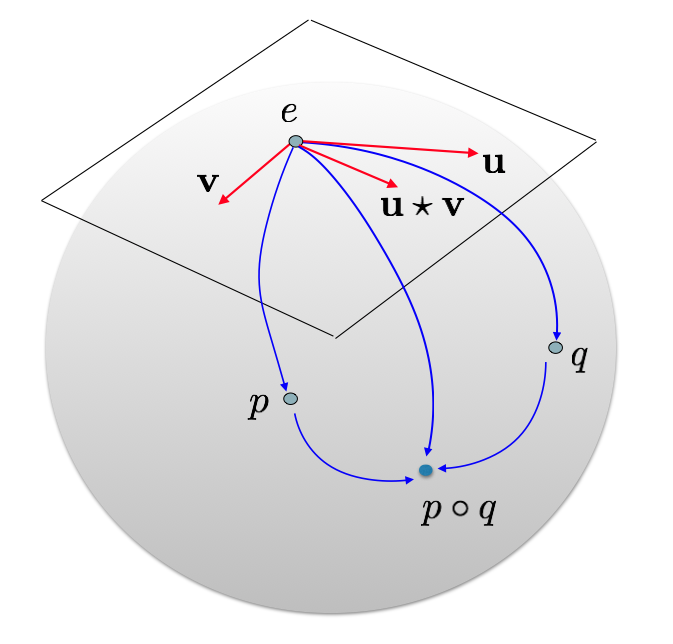
\includegraphics[scale=0.35]{figures/log_composition.png}
	\caption{graphical visualization of the Lie log-composition.}
	\label{fig:composition}
\end{figure}

\noindent
Following properties holds for the Lie log-composition:
\begin{enumerate}
	\item $\mathfrak{g} $ with the Lie log-composition $\oplus$ is a local topological non-commutative group (local group for short): if $C_{\mathfrak{g}}$ is the internal cut locus of $\mathfrak{g}$ then:
	\begin{enumerate}
		\item $(\mathbf{u}_{1}\oplus\mathbf{u}_{2}) \oplus \mathbf{u}_{3}
		= \mathbf{u}_{1}\oplus(\mathbf{u}_{2} \oplus \mathbf{u}_{3})$ for all $\mathbf{u}_{1}, \mathbf{u}_{2}, \mathbf{u}_{3}$ in $C_{\mathfrak{g}}$.
		\item $\mathbf{u}\oplus\mathbf{0}  = \mathbf{0}\oplus\mathbf{u} = \mathbf{u}$ for all $\mathbf{u}$ in $C_{\mathfrak{g}}$.
		\item $\mathbf{u}\oplus(-\mathbf{u} ) = \mathbf{0}$ for all $\mathbf{u}$ in $C_{\mathfrak{g}}$.
	\end{enumerate}
	\item For all $t,s$ real, such that $(t+s)\mathbf{u}$ is in $C_{\mathfrak{g}}$,
	\begin{align*}
	(t\mathbf{u})\oplus (s\mathbf{u}) = (t+s)\mathbf{u}
	\end{align*}
	And in particular, if the Lie algebra $\mathfrak{g}$ has dimension $1$ the local group structure is compatible with the additive group of the vector space $\mathfrak{g}$.
\end{enumerate}

\noindent
The algebraic structure $(\mathfrak{g} , \oplus)$ is called Lie log-group. Additional observations on this algebraic structure in the particular case of diffeomorphisms, are proposed in the next chapter.\\
To compute the log-composition there is a formula, the BCH (for matrix Lie group \cite{hall2015lie}, general case \cite{wojtynski1994one}, applied to medical imaging \cite{vercauteren08}), that provides the exact solution to the Log-composition. 
\begin{align*}
BCH(\mathbf{u},\mathbf{v}) 
= 
\mathbf{u} + \mathbf{v} + \frac{1}{2}[\mathbf{u},\mathbf{v}] + \frac{1}{12}([\mathbf{u},[\mathbf{u},\mathbf{v}]]
+ [\mathbf{v},[\mathbf{v},\mathbf{u}]]) - \frac{1}{24}[\mathbf{v},[\mathbf{u},[\mathbf{u},\mathbf{v}]]] +... 
\end{align*}
This expansion will provide the most immediate way to obtain a numerical computation of $\mathbf{v}_{1}\oplus \mathbf{v}_{2}$.

%
%% % % % % % % % % % % % % % % % % % % % % % % % % % % % % % % % % % % % % %
%% % SECTION
%% % % % % % % % % % % % % % % % % % % % % % % % % % % % % % % % % % % % % % 
%\section{Affine Exponential, Affine logarithm and affine log-composition}\label{se:affine_exp_log_comp}
%


% % % % % % % % % % % % % % % % % % % % % % % % % % % % % % % % % % % % % %
% % SECTION
% % % % % % % % % % % % % % % % % % % % % % % % % % % % % % % % % % % % % % 
\section{Affine Exponential, Affine Logarithm and Parallel Transport: Definition and Properties}\label{se:parallel_transport}

Considering a Lie Group $\mathbb{G}$ with a connection $\nabla$ (that provides geodesics and curvature over manifold on which no Riemannian metric has been defined, see \cite{do1992riemannian}), the vector field $\nabla_{U}(V)$ associates at each point of the manifold the projection on the tangent plane of the covariant derivative of $U$ in the direction of $V$. \\
First consequence of the definition of the connection is the possibility of define \emph{geodesics} between points $p$ and $q$ of the manifold. 
Note that in this case the concept of geodesic does not involves any metric defined on the surface of the manifold. If also a Riemannian metric is defined on $\mathbb{G} $, then geodesics defined by the metric coincides with the geodesics defined by the connection only for the particular Levi-Civita connection (see \cite{do1992riemannian}).

Another consequence of the definition of connection allows to define a new kind of exponential from the Lie algebra to the Lie group that relies on the concept of geodesics. This time the tangent plane that defines the Lie algebra is considered at the point $p$ of the Lie group and $\mathbf{v} \in T_{p}\mathbb{G}\simeq \mathfrak{g}$ is a tangent vector at the point $p$: 
\begin{align*}
\exp :  \mathbb{G}  \times \mathfrak{g}     &\longrightarrow \mathbb{G}  
\\ 
(p,\mathbf{v}) &\longmapsto \exp_{p}(\mathbf{v})  = \gamma(1; p,\mathbf{v})
\end{align*}
The curve $\gamma(t;p,\mathbf{v}) = \gamma(t)$ on $\mathbb{G}$ is the unique one with the following features:  
\begin{align*}
\gamma(0) = p\qquad  \dot{\gamma}(0) =  \mathbf{v} \qquad \nabla_{\dot{\gamma}}\dot{\gamma} = 0 
\end{align*}
This second kind of exponential is called \emph{affine exponential}.\\

\noindent
The inverse of the affine exponential, the affine logarithm is defined as:
\begin{align*}
\log :  \mathbb{G}  \times \mathbb{G}   \longrightarrow T_{p}\mathbb{G}   \simeq \mathfrak{g} 
\\ 
(p,q) \longmapsto \log_{p}(q)  = \mathbf{v} 
\end{align*}
Where $\mathbf{v} $ is the vector at the tangent plane defined at $p$ such that the curve on $\mathbb{G} $ with the following features
\begin{align*}
\gamma(0) = p\qquad  \gamma(1) = q \qquad \nabla_{\dot{\gamma}}\dot{\gamma} = 0 
\end{align*}
has as its tangent in $p$ the vector $\mathbf{v}$.\\

For further details and properties properties we refer to the literature; here we wish to provide only the intuitive idea that it is possible to move on the fiber bundle of the Lie group transporting in some sense a tangent vector defined at the identity on another tangent space. Certainly the Lie group possess a unique Lie algebra, as the tangent space at some point (the group's identity by convention), but two different tangent space (so two times the same Lie algebra structure) may not be oriented in the same way. \\

In this section we introduce the concept of parallel transport for the Lie group $\mathbb{G}$. On this definition, again borrowed from differential geometry (for introduction and general definition: \cite{misner1973gravitation}, \cite{knebelman1951spaces}, \cite{kheyfets2000schild} and \cite{warner} for a definition of tangent vector field well suited for the parallel transport. For medical imaging applications \cite{lorenzi2011schild}, \cite{pennec2011parallel}, \cite{lorenzi2013geodesics}, \cite{lorenzi2014efficient}), relies a method for the computation of the log-composition developed in this research for the first time.

\begin{definition}
	Let $\mathbb{G}$ be a finite dimensional connected Lie group defined with a connection $\nabla$ and $V$ a $\mathcal{C}^{\infty}$ vector field defined over $\mathbb{G}$. Given $p,q \in \mathbb{G}$ and $\gamma : [0,1] \rightarrow \mathbb{G}$ such that $\gamma(0) = p$ and $\gamma(1) = q$, the vector $V_{p} \in T_{p}\mathbb{G}$, is \emph{parallel transported along $\gamma$} up to $T_{q}\mathbb{G}$ if $V$ satisfies
	\begin{align*}
	\forall t \in  [0,1]
	\qquad
	\nabla_{\dot{\gamma}}V_{\gamma(t)} = 0
	\end{align*}
	The \emph{parallel transport} is the function that maps $V_{p}$ from $T_{p}\mathbb{G}$ to $T_{q}\mathbb{G}$ along $\gamma$:
	\begin{align*}
	\Pi(\gamma)_{p}^{q} :  T_{p}\mathbb{G} & \longrightarrow T_{q}\mathbb{G}  \\
	V_{p}&\longmapsto \Pi(\gamma)_{p}^{q}(V_{p}) = V_{q}
	\end{align*}
\end{definition}
\noindent
In the next properties we explore how did parallel transport and affine exponential behave when expressed as a composition and when the signs change.
\begin{prop}[Inversion]
	$\mathbb{G}$ Lie group, $\nabla$ connection, $p,q\in\mathbb{G}$. Given $\gamma$ such that $\gamma(0)= p$, $\gamma(1)=q$ and $\mathbf{u}\in T_{p}\mathbb{G}$, we have:
	\begin{enumerate}
	\item $\Pi(\gamma)_{p}^{q}(-\mathbf{u}) = -\Pi(\gamma)_{p}^{q}(\mathbf{u}) )$
	\item $q = \exp_{p}(\mathbf{u}) \phantom{z} \Longleftrightarrow \phantom{z} p = \exp_{q}(-\Pi(\gamma)_{p}^{q}(\mathbf{u}))$
	\end{enumerate}
\end{prop}

\begin{figure}[htbp]
	\centering
	\begin{minipage}[b]{3cm}
		\hspace{-4cm}
		\centering
		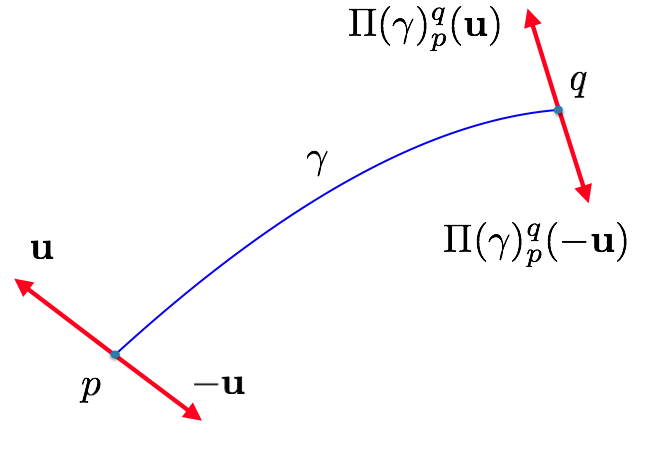
\includegraphics[width=6.5cm]{figures/inversion_1.png}
		\caption{First inversion property.}
		\label{fig:inversion_propr1}
	\end{minipage}
	\ \hspace{9mm} \
	\begin{minipage}[b]{4cm}
		\centering
		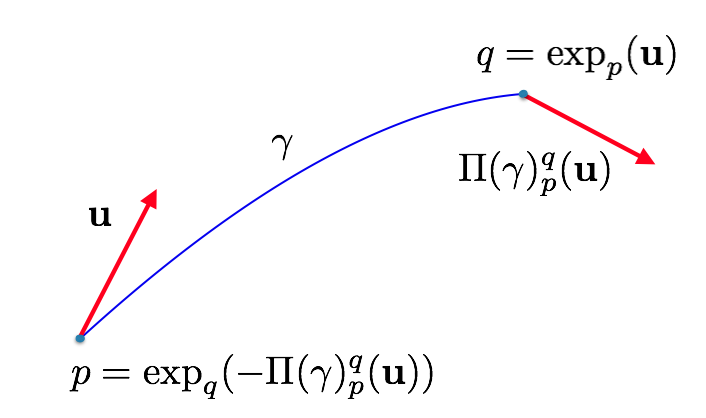
\includegraphics[width=6.5cm]{figures/inversion_2.png}
		\caption{Second inversion property.}
		\label{fig:inversion_propr2}
	\end{minipage}
\end{figure}
\begin{prop}[change of signs of the composition for affine exponential]
	$\mathbb{G}$ Lie group, $\nabla$ connection, $p,q\in\mathbb{G}$, $\mathbf{u}\in T_{p}\mathbb{G}$, $\mathbf{v}\in T_{q}\mathbb{G}$ and $q=\exp_{p}(\mathbf{u})$. Let $\beta$ be the tangent curve to $\mathbf{u}$ at $p$ such that $\beta(1) = q$ and $r= \exp_{b}(\mathbf{v})$. Given $\mathbf{w} \in T_{p}\mathbb{G}$ such that 
	\begin{align*}
	\exp_{p}(\mathbf{w}) = \exp_{q}(\mathbf{v}) \circ \exp_{p}(\mathbf{u})
	\end{align*}
	Then
	\begin{align*}
	\exp_{p}(-\mathbf{w}) = \exp_{\beta(-1)}(-\Pi(\beta)_{q}^{\beta(-1)}(\mathbf{v})) \circ \exp_{p}(-\mathbf{u})
	\end{align*}
\end{prop}

\begin{figure}[htbp]
	\centering
	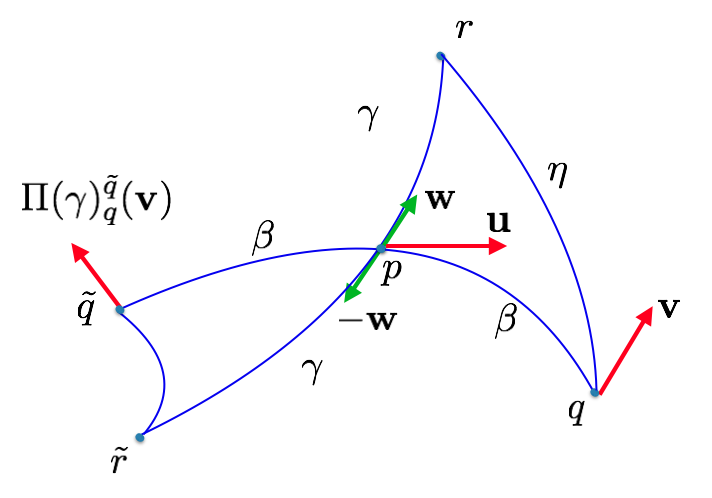
\includegraphics[width=9.5cm]{figures/sign_1.png}
	\caption{Change of sign property.}
	\label{fig:sign_propr}
\end{figure}

\begin{lemma}
	Let $\mathbb{G}$ be a finite dimensional connected Lie group defined with a Cartan connection $\nabla$ and $\mathbf{u}$ tangent vector in $ T_{e}\mathbb{G}$. Let $\gamma$ be a geodesic defined on $\mathbb{G}$ such that $\gamma(0) = e$, $\dot{\gamma}(0) =\mathbf{u}$ and $p = \gamma(1)$, point in the Lie group. Let $\beta$ be the curve over $\mathbb{G}$ defined as $\beta(t) = p\circ \gamma(t)$, then the two following conditions hold:
	\begin{enumerate}
		\item If $\nabla$ is a Cartan connection then $\beta$ is a geodesic.
		\item For $\mathbf{u}_{p} := D(L_{p})_{e}(\mathbf{u}) \in T_{p}\mathbb{G}$, push forward of the left-translation:
		\begin{align}\label{eq:lemma_pt}
		\exp_{p}(t\mathbf{u}_{p}) = p\circ \exp_{e}( t D(L_{p^{-1}})_{p}(\mathbf{u}_{p}) ) 
		= p\circ \exp_{e}(t\mathbf{u})
		\end{align}
	\end{enumerate}
\end{lemma}

\begin{figure}[htbp]
	\centering
	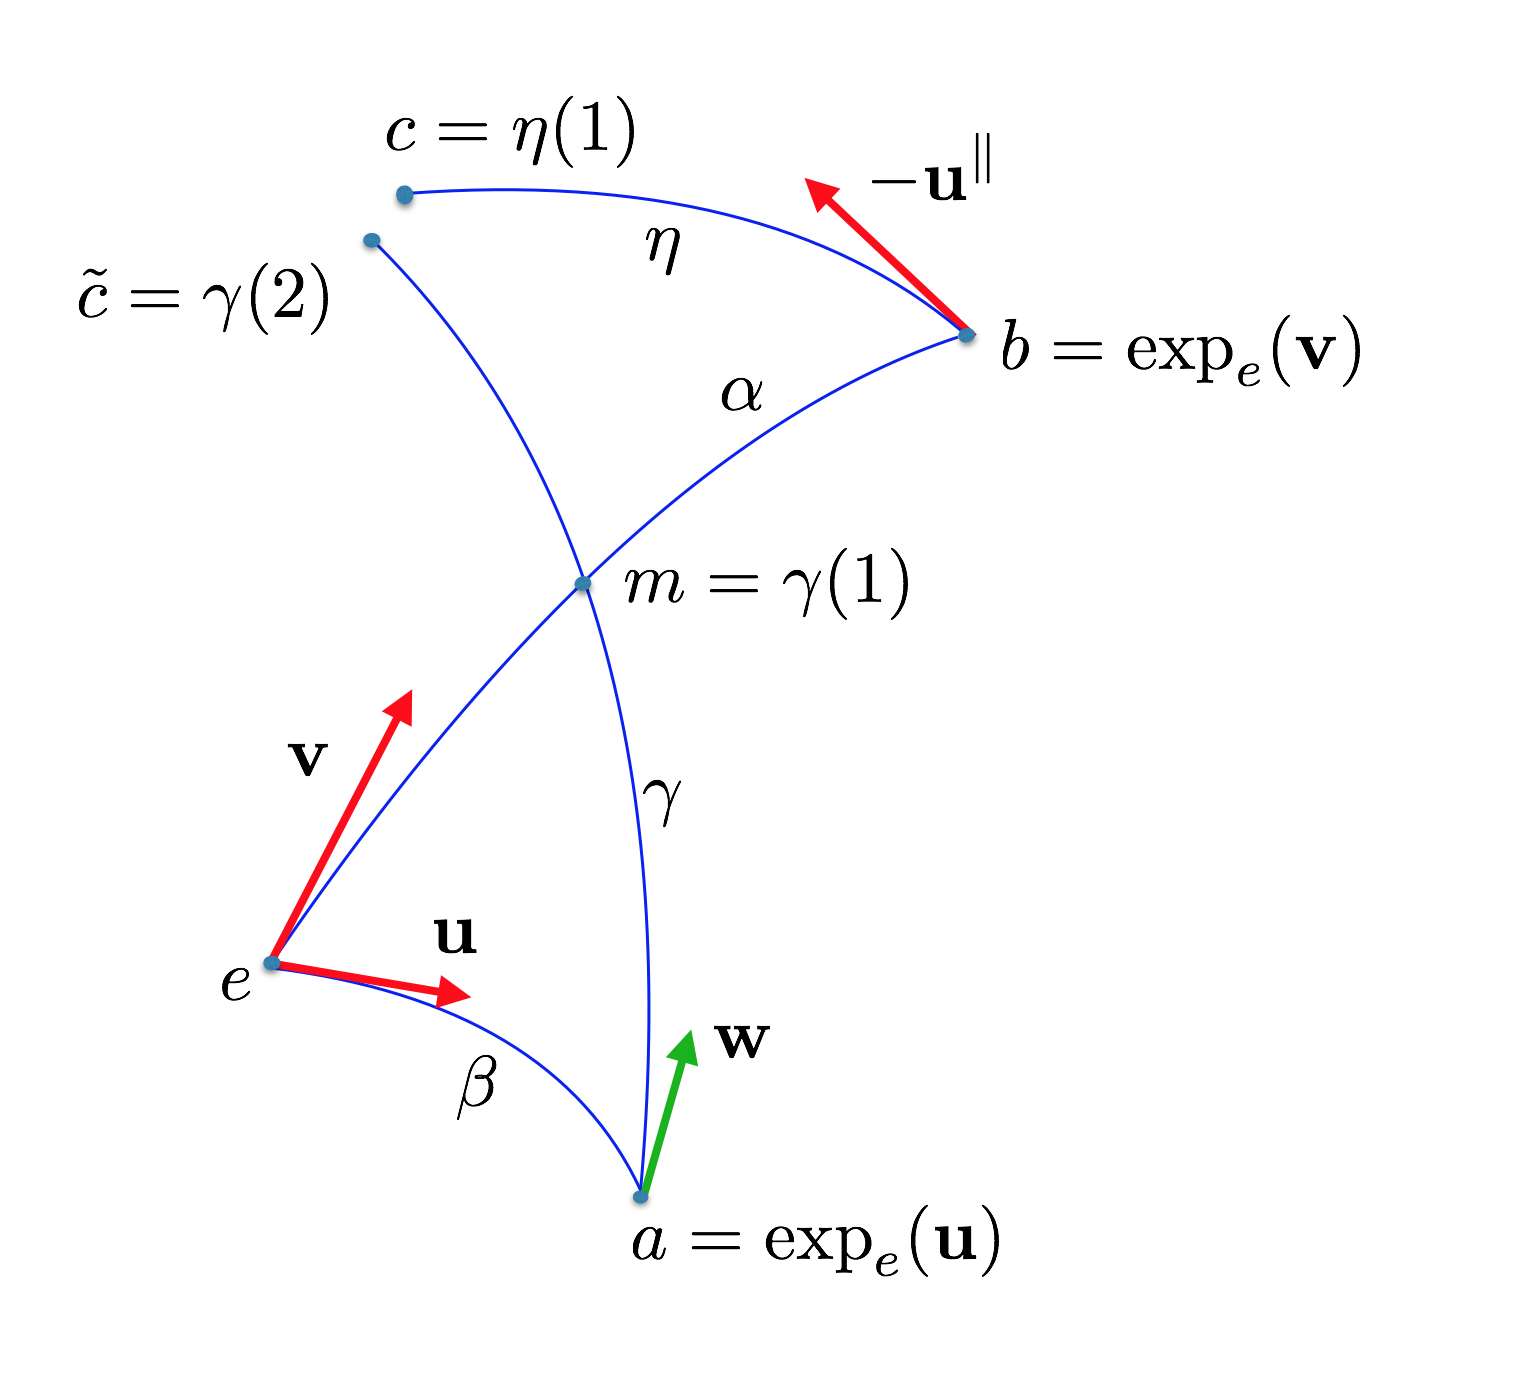
\includegraphics[width=9.5cm]{figures/theorem_pict.png}
	\caption{Pole ladder applied to parallel transport.}
	\label{fig:theorem_pict}
\end{figure}
\noindent
The following theorem is an application of the pole ladder \cite{lorenzi2011schild} for the computation of the exponential that will underpin one of the numerical methods for the computation of the log-composition.
\begin{theorem}\label{th:local_approximation_theorem}
	Let $\mathbb{G}$ be a finite dimensional connected Lie group defined with a Cartan connection $\nabla$. 
	If, for each couple of linearly independent vectors $\mathbf{u}, \mathbf{v} \in T_{e}\mathbb{G}$, the following conditions hold:
	\begin{align*}
	a = \exp_{e}(\mathbf{u}) 
	\quad & \quad  
	b = \exp_{e}(\mathbf{v}) \\
	\mathbf{v}_{a}^{\parallel} = & \Pi(\gamma)_{e}^{a}(\mathbf{v})\\
	\gamma : [0,1] \rightarrow \mathbb{G} &\quad \gamma(0) = e \quad \dot{\gamma}(0) = \mathbf{u}
	\end{align*}
	\begin{align*}
	 \mathbf{v}^{\parallel} := D(L_{a^{-1}})_{e}( -\Pi(\alpha)_{a}^{e}(\mathbf{v}_{a}^{\parallel}))
	\end{align*}
	Then it follows that if $\mathbf{u}$ is in the open ball $B(\mathbf{0}, \epsilon)$, then exists a  $\tilde{\epsilon}>0$ such that $\mathbf{u}_{e}^{\parallel}$ belongs to $B(\mathbf{0}, \tilde{\epsilon})$, and exists a $\delta(\epsilon + \tilde{\epsilon})>0$ such that the inequality
	\begin{align*}
		\euclideanMetric{
			\log(\exp_{e}(\mathbf{v}^{\parallel} ))
			-
			\log(\exp_{e}\big(\frac{\mathbf{u}}{2}\big)   
				\circ  \exp_{e}(\mathbf{v}) 
				\circ \exp_{e}\big(-\frac{\mathbf{u}}{2}\big))
			} <\delta(\epsilon + \tilde{\epsilon})
	\end{align*}
	holds.
\end{theorem}
\noindent
The last statement can be rewritten as the approximation:
\begin{align}\label{eq:parallel_transport_main_approximation}
\exp_{e}(\mathbf{v}^{\parallel}) 
\simeq
\exp_{e}\big(\frac{\mathbf{u}}{2}\big)   
\circ  \exp_{e}(\mathbf{v}) 
\circ \exp_{e}\big(-\frac{\mathbf{u}}{2}\big)
\end{align}
that will turn out to be the main tool for the computation of the log-composition using parallel transport.


% % % % % % % % % % % % % % % % % % % % % % % % % % % % % % % % % % % % % %
When considering the equation \ref{eq:lemma_pt}, we use implicitly the formula for the change of base for affine exponential and logarithm \cite{arsigny2006bi}. It is in fact possible, using the derivative of the left-translation $L_{p}$, to bring back the $\exp$ and the $\log$ functions based at the point $p$ of the manifold to the $\exp$ and the $\log$ evaluated at the identity using the following formulas:
\begin{align}\label{eq:DL_DR}
\log _{p}(q)  &= DL_{p}(e) \log _{e}(q)  \\
\exp _{p}(\mathbf{u})  &= p\circ \exp_{e} (DL_{p}(e)^{-1} \mathbf{u})
\end{align}
\noindent
Further theoretical developments are beyond the aim of this research, but the reader can refer to the bibliography.
In the next section we present the numerical methods for the computation of the log composition.



% % % % % % % % % % % % % % % % % % % % % % % % % % % % % % % % % % % % % %
% % SECTION
% % % % % % % % % % % % % % % % % % % % % % % % % % % % % % % % % % % % % %
\section{Numerical Computations of the Log-composition}

In this section we provide explicit formulas for the computation of the log composition:
\begin{align}\label{eq:general_numerical_log_composition}
\mathbf{v}_{1}\oplus \mathbf{v}_{2} =  \log(\exp(\mathbf{v}_1)\circ \exp(\mathbf{v}_2))
\end{align}
using the tools introduced in the previous sections.

% % % % % % % % % % % % % % % % % % % % % % % % % % % % % % % % % % % % % %
% % SUBSECTION
% % % % % % % % % % % % % % % % % % % % % % % % % % % % % % % % % % % % % % 
\subsection{Truncated BCH formula for the Log-composition}\label{se:bch_formula}

To compute the Lie log-composition, literature provides the BCH formula (for matrices \cite{hall2015lie}, general case: \cite{klarsfeld1989baker} , \cite{serre2009lie}), defined as the solution of the equation $\exp(\mathbf{w}) = \exp(\mathbf{u}) \circ \exp(\mathbf{v})$, for $\bf{u}$ and $\bf{v}$ in the Lie algebra $\mathfrak{g}$:
\begin{align}\label{eq:bch_definition}
	BCH(\mathbf{u},\mathbf{v}) 
	= 
	\mathbf{u} + \mathbf{v} + \frac{1}{2}[\mathbf{u},\mathbf{v}] + \frac{1}{12}([\mathbf{u},[\mathbf{u},\mathbf{v}]]
	+ [\mathbf{v},[\mathbf{v},\mathbf{u}]]) - \frac{1}{24}[\mathbf{v},[\mathbf{u},[\mathbf{u},\mathbf{v}]]] +... 
\end{align}
It consists of an infinite series of Lie bracket whose asymptotic behaviour cannot be predicted only from the coefficient of each nested Lie bracket term. In practical applications it can be computed using its \emph{approximation of degree} $k$, defined as the sum of the BCH terms having no more than $k$ nested Lie bracket. For example:
\begin{align*}
BCH^{0}(\mathbf{u},\mathbf{v}) &= \mathbf{u} + \mathbf{v} \\
BCH^{1}(\mathbf{u},\mathbf{v}) &=  \mathbf{u} + \mathbf{v} + \frac{1}{2}[\mathbf{u},\mathbf{v}] \\
BCH^{2}(\mathbf{u},\mathbf{v}) &=  \mathbf{u} + \mathbf{v} + \frac{1}{2}[\mathbf{u},\mathbf{v}] + \frac{1}{12}([\mathbf{u},[\mathbf{u},\mathbf{v}]] + [\mathbf{v},[\mathbf{v},\mathbf{u}]]) \\
BCH^{3}(\mathbf{u},\mathbf{v}) &=  \mathbf{u} + \mathbf{v} + \frac{1}{2}[\mathbf{u},\mathbf{v}] + \frac{1}{12}([\mathbf{u},[\mathbf{u},\mathbf{v}]] + [\mathbf{v},[\mathbf{v},\mathbf{u}]])- \frac{1}{24}[\mathbf{v},[\mathbf{u},[\mathbf{u},\mathbf{v}]]] 
\end{align*}
These numerical approximations of the log-composition $\mathbf{u}\oplus \mathbf{v}$ can be considered as a first step but are not satisfactory since they do not provide any condition to consider the error carried by each term.


% % % % % % % % % % % % % % % % % % % % % % % % % % % % % % % % % % % % % %
% % SUBSECTION
% % % % % % % % % % % % % % % % % % % % % % % % % % % % % % % % % % % % % % 
\subsection{Taylor Expansion Method for the Log-composition}\label{se:taylor_expansion}

A more sophisticated numerical method to manage the nested Lie brackets for the computation of the log-composition is based on the Taylor expansion. \\
As shown in the appendix of \cite{klarsfeld1989baker} the terms of the BCH can be recollected using the Hausdorff method: each of the therm containing the n-th power of the vector $\mathbf{v}$ are collected together in the formal series $V^{n}$. Therefore
\begin{align*}
%\mathbf{u}\oplus \mathbf{v}  
BCH(\mathbf{u},\mathbf{v}) 
= 
\mathbf{u} + V^{1} \mathbf{v} + V^{2} \mathbf{v} + V^{3} \mathbf{v} + \cdots
\end{align*}
Given the adjoint map:
\begin{align*}
ad_{\mathbf{u}} : \mathfrak{g}  & \longrightarrow \mathfrak{g}  
\\
\mathbf{v} &\longmapsto ad_{\mathbf{u}}   \mathbf{v} :=  [\mathbf{u}, \mathbf{v}]
\end{align*}
and the multiple adjoint maps, defined as:
\begin{align*}
\text{ad}_{\mathbf{u}}^{n} \mathbf{v} 
&:= [  \underbrace{   \mathbf{u},[\mathbf{u},... [\mathbf{u}}_{\text{n-times}},\mathbf{v}]...]] 
\\
\\
\text{ad}_{\mathbf{u}}^{-n} \mathbf{v} 
&:= [[...[  \mathbf{v}, \underbrace{   \mathbf{u}]...],\mathbf{u}}_{\text{n-times}}]
= (-1)^n \text{ad}_{\mathbf{u}}^{n} \mathbf{v} 
\end{align*}
it can be proved that hen the operator $V^{1}$ is applied to $\mathbf{v}$, it provides the linear part of $\mathbf{v}$ in the BCH formula. It results
\begin{align*}
V_{1}
= 
\frac{  
	\text{ad}_{\mathbf{u}}^{-1} 
	}{
	\exp{(\text{ad}_{\mathbf{u}})}-1
	}
=
\sum_{n=0}^{\infty} \frac{(-1)^nB_{n}}{n!} \text{ad}_{\mathbf{u}}^{ - n} 
=
\sum_{n=0}^{\infty} \frac{B_{n}}{n!} \text{ad}_{\mathbf{u}}^{ n} 
\end{align*}
where $\lbrace B_{n} \rbrace_{n=0}^{\infty} $ is the sequence of the second-kind Bernoulli number. If first-kind Bernoulli number are used, then each term of the summation must be multiplied for $(-1)^{n}$, as did for example in \cite{klarsfeld1989baker}. The denominator is defined within the structure of the formal power series ring \cite{mariconda2013calcolo}.\\
In conclusion, the log-composition can expressed as:
\begin{align*}
\mathbf{u}\oplus \mathbf{v}  
&= 
\mathbf{u} + 
\frac{  
	\text{ad}_{\mathbf{u}}^{-1} 
}{
\exp{(\text{ad}_{\mathbf{u}})}-1
} \mathbf{v}  
+ 
\mathcal{O}(\mathbf{v} ^2) 
\end{align*}
\begin{align}\label{eq:taylor}
\mathbf{u}\oplus \mathbf{v}  
&=
\mathbf{u} 
+
\sum_{n=0}^{\infty} \frac{B_{n}}{n!} \text{ad}_{\mathbf{u}}^{ n} 
\mathbf{v}  
+
\mathcal{O}(\mathbf{v} ^2)
\end{align}
that will turn out to be an important tool for the computation of the log-composition in the finite dimensional case. \\


% % % % % % % % % % % % % % % % % % % % % % % % % % % % % % % % % % % % % %
% % SUBSECTION
% % % % % % % % % % % % % % % % % % % % % % % % % % % % % % % % % % % % % % 
\subsection{Parallel Transport Method for the Log-composition}
To obtain a numerical computation for the log-composition using parallel transport, we have to consider two assumptions: 
\begin{enumerate}
	\item If $\mathbf{v}^{\parallel} $ is defined as in theorem \ref{th:local_approximation_theorem}, then exists an $\hat{\epsilon} > 0$ such that
	\begin{align*}
	\euclideanMetric{
		\mathbf{u}\oplus \mathbf{v}  
		-
		(
		\mathbf{u} + \mathbf{v}^{\parallel} 
		)
	} <\hat{\epsilon}
	\end{align*}
	\item If the vector $\mathbf{w}\in\mathfrak{g}$ is small enough, then:
		\begin{align*}
		\exp(\mathbf{u}) \simeq e + \mathbf{u}
		\end{align*}
\end{enumerate}
The first assumption is a consequence of geometrical intuition, while
the second one is valid if the hypothesis of proposition 8.6 pag. 163 \cite{younes2010shapes} holds. A deepening in this direction is not in the scope of this research. For our purposes we will consider the vector $\mathbf{w}$ small enough to make the approximation questioned here reasonable.\\

From these assumptions and from equation \ref{eq:parallel_transport_main_approximation} it follows that 
\begin{align*}
\mathbf{u}\oplus \mathbf{v}
&\simeq
\mathbf{u} + \mathbf{v}^{\parallel}
\\
e + \mathbf{v}^{\parallel}
&\simeq
\exp_{e}\big(\frac{\mathbf{u}}{2}\big)   
\circ  \exp_{e}(\mathbf{v}) 
\circ \exp_{e}\big(-\frac{\mathbf{u}}{2}\big)
\end{align*}
Therefore
\begin{align}\label{eq:parallel_transport}
\mathbf{u}\oplus \mathbf{v}
&\simeq
\mathbf{u} 
+
\exp_{e}\big(\frac{\mathbf{u}}{2}\big)   
\circ  \exp_{e}(\mathbf{v}) 
\circ \exp_{e}\big(-\frac{\mathbf{u}}{2}\big)
 -
 e
\end{align}
With the truncated BCH and the Taylor expansion, this is the third numerical method for the computation of the log-composition explored in this thesis.\\
We have to notice that when we apply it on the infinite dimensional case, the approximation \ref{eq:parallel_transport} holds under the following additional assumption:
\begin{enumerate}
\item[3.] Theorem \ref{th:local_approximation_theorem} holds when the Lie group is infinite dimensional.
\end{enumerate}
An eventual confirmation is at the moment not known to the author. We assume it is true in coherence with what has been said in the introduction, section \ref{se:diffe_util_and_liab}.











\chapter{Spatial Transformations for the Computations of the Log-composition: $SE(2)$ and $\text{Diff}(\Omega)$}\label{ch:spatial_transformations}


\begin{flushright}
	\emph{Every working mathematician knows that if one does not control oneself (best of all by examples), then after some ten pages half of all the signs in formulae will be wrong and twos will find their way from denominators into numerators. \\ -V.I. Arnold}
\end{flushright}

\noindent
In the previous chapter we have introduced some essential mathematical tools for the numerical computation of the log-composition. Each of the theoretical elements depends strongly on the transformations considered, and in this chapter we will see how they can be applied for the transformations belonging to $SE(2)$ and $\text{Diff}(\Omega)$.
%\begin{enumerate}
%	\item[$SE(2)$ -] The group of rigid body transformation of the plane (any combination of bi-dimensional rotations and translations) is a good playground to test the numerical methods for the computation of the log-composition introduced so far, since results can be compared with a ground truth.
%	\item[$\text{Diff}(\Omega)$ -] The group of diffeomorphisms over $\Omega$, indcated with $\text{Diff}(\Omega)$ is defined over the wide set of all of the differentiable and invertible functions. For our applications we will restrict the set to the diffeomorphisms that can be parametrized by stationary velocity fields or SVF. This infinite dimensional vector space is the second algebra utilized to test the numerical methods for the computation of the log-composition. In this case we do not know any closed form, but considering an \lq\lq improper norm\rq\rq~ in the space of deformations it is possible to compare SVF and assess the quality of the results.
%\end{enumerate}


\section{The Lie Group of Rigid Body Transformations}\label{se:rigid_body_transformations}
% group
Each element of the group of rigid body transformation (or euclidean group) $SE(2)$ can be computed as the consecutive application of a rotation and a translation applied to any point $(x,y)^T$ of the plane:
\begin{align*}
\left (  
\begin{array} {c }
X \\
Y
\end{array}
\right )  
= 
R(\theta)
\left (  
\begin{array} {c }
x \\
y
\end{array}
\right ) 
+
t
=
\left (
\begin{array} {c c }
\cos(\theta) & - \sin(\theta) \\
\sin(\theta) & \cos(\theta) 
\end{array}
\right )
\left (  
\begin{array} {c }
x \\
y
\end{array}
\right ) 
+
\left (  
\begin{array} {c }
t^x \\
t^y
\end{array}
\right ) 
\end{align*}
where the rotation matrix indicated with $R(\theta)$ belongs to the special orthogonal group $SO(2)$ and the translation $t$ is a vector of the plane.\\
We can represent the elements of $SE(2)$ in two different form: as ternary vector (restricted form) 
\begin{align*}
SE(2)^{v} 
:=
\{ (\theta, t^x, t^y) \mid \theta \in [0, 2\pi),   t^x, t^y \in\mathbf{R}^2  \}
\end{align*}
or with matrices (matrix form)
\begin{align*}
SE(2) 
:= 
\left \{
\left (
\begin{array} {c c }
R(\theta) & t \\
0 & 1 
\end{array}
\right )
=
\left (
\begin{array} {c c c }
\cos(\theta) & - \sin(\theta)& t^{x} \\
\sin(\theta) & \cos(\theta) & t^{y}\\
0 & 0 &  1
\end{array}
\right )
\mid
\theta \in  [0, 2\pi), (t^x, t^y) \in\mathbf{R}^2
\right \}
\end{align*}
The group $SE(2)$ it is a manifold with a differentiable structure compatible with the operation of composition, whose Lie algebra is given in matrix form by
\begin{align*}
\mathfrak{se}(2) := 
\left \{
\left (
\begin{array} {c c }
dR(\theta) & dt \\
0 & 0
\end{array}
\right )
=
\left (
\begin{array} {c c c }
0 & -\theta &  dt^{x} \\
\theta & 0 & dt^{y} \\
0& 0 & 0
\end{array}
\right )
\mid
\theta \in  [0, 2\pi), (dt^x, dt^y) \in\mathbf{R}^2
\right \}
\end{align*}
and it is indicated with $\mathfrak{se}(2)^{v}$ in its restricted form.

Given $r$, element of $SE(2)$ with $\theta\neq 0$, its image with the Lie group logarithm is
\begin{align*}
\log(r)
&=
\sum_{k=1}^{\infty} (-1)^{k+1}~\frac{(r - I)^k}{k}
=
\left (
\begin{array} {c c }
dR(\theta) & L(\theta)t \\
0 & 1 
\end{array}
\right )
\\
&=
\left (
\begin{array} {c c c}
0   & - \theta& \frac{\theta}{2} (\frac{\sin(\theta)}{1-\cos(\theta)} t^x + t^y )\\
\theta & 0     & \frac{\theta}{2} (- t^x + \frac{\sin(\theta)}{1-\cos(\theta)} t^y )\\
0 & 0 &  0
\end{array}
\right )
\end{align*}
where 
\begin{align*}
dR(\theta) = 
\left (
\begin{array} {c c }
0 & -\theta \\
\theta & 0 
\end{array}
\right )
\qquad \qquad 
L(\theta) = 
\frac{\theta}{2}
\left (
\begin{array} {c c }
\frac{\sin(\theta)}{1-\cos(\theta)} & 1 \\
-1 & \frac{\sin(\theta)}{1-\cos(\theta)}
\end{array}
\right )
\end{align*}
On the way back, the exponential of $dr \in \mathfrak{se}(2)$ is given by:
\begin{align*}
\exp(dr)
&=
\sum_{k=1}^{\infty} \frac{dr^{k}}{k!}
=
\left (
\begin{array} {c c }
R(\theta) & L(\theta)^{-1}dt \\
0 & 1 
\end{array}
\right )
\\
&=
\left (
\begin{array} {c c c}
\cos(\theta)   & - \sin(\theta)& \frac{1}{\theta} (\sin(\theta)dt^x - (1-\cos(\theta)) dt^y )\\
\sin(\theta) & \cos(\theta)     & \frac{1}{\theta} (- (1-\cos(\theta))dt^x + \sin(\theta) dt^y )\\
0 & 0 &  1
\end{array}
\right )
\end{align*}
where
\begin{align*}
L(\theta)^{-1} = 
\frac{1}{\theta}
\left (
\begin{array} {c c }
\sin(\theta) & -(1-\cos(\theta)) \\
(1-\cos(\theta)) & \sin(\theta)
\end{array}
\right )
\end{align*}
When $\theta$ is zero, $R(\theta)$ and $dR(\theta)$ coincide with the identity, and the transformation results in a translation. For proof and further details see for example \cite{gallier2011geometric} \cite{hall2015lie}.

At this point it is important to notice that: 
\begin{enumerate}
	%infinite series 
	\item The infinite series of matrices  do not raises any theoretical issues, since the sum is defined in the group as subset of a bigger algebra that contains both the Lie group and the Lie algebra. It appears to be the natural way to move back and forth from the group to the algebra. A second door to passing from one structure to the other, when the rotation $\theta$ is small is provided by the following approximations:
	\begin{align}\label{eq:small_rotation_matrices_approx}
	\exp(r) \simeq I + r
	\qquad 
	\log(dr) \simeq dr - I
	\end{align}
	In fact for small $\theta$, $\sin(\theta) \simeq \theta$, $\cos(\theta) \simeq 0 $ and $ L(\theta) \simeq I$.
   %
	\begin{figure}[!ht]
		\centering
		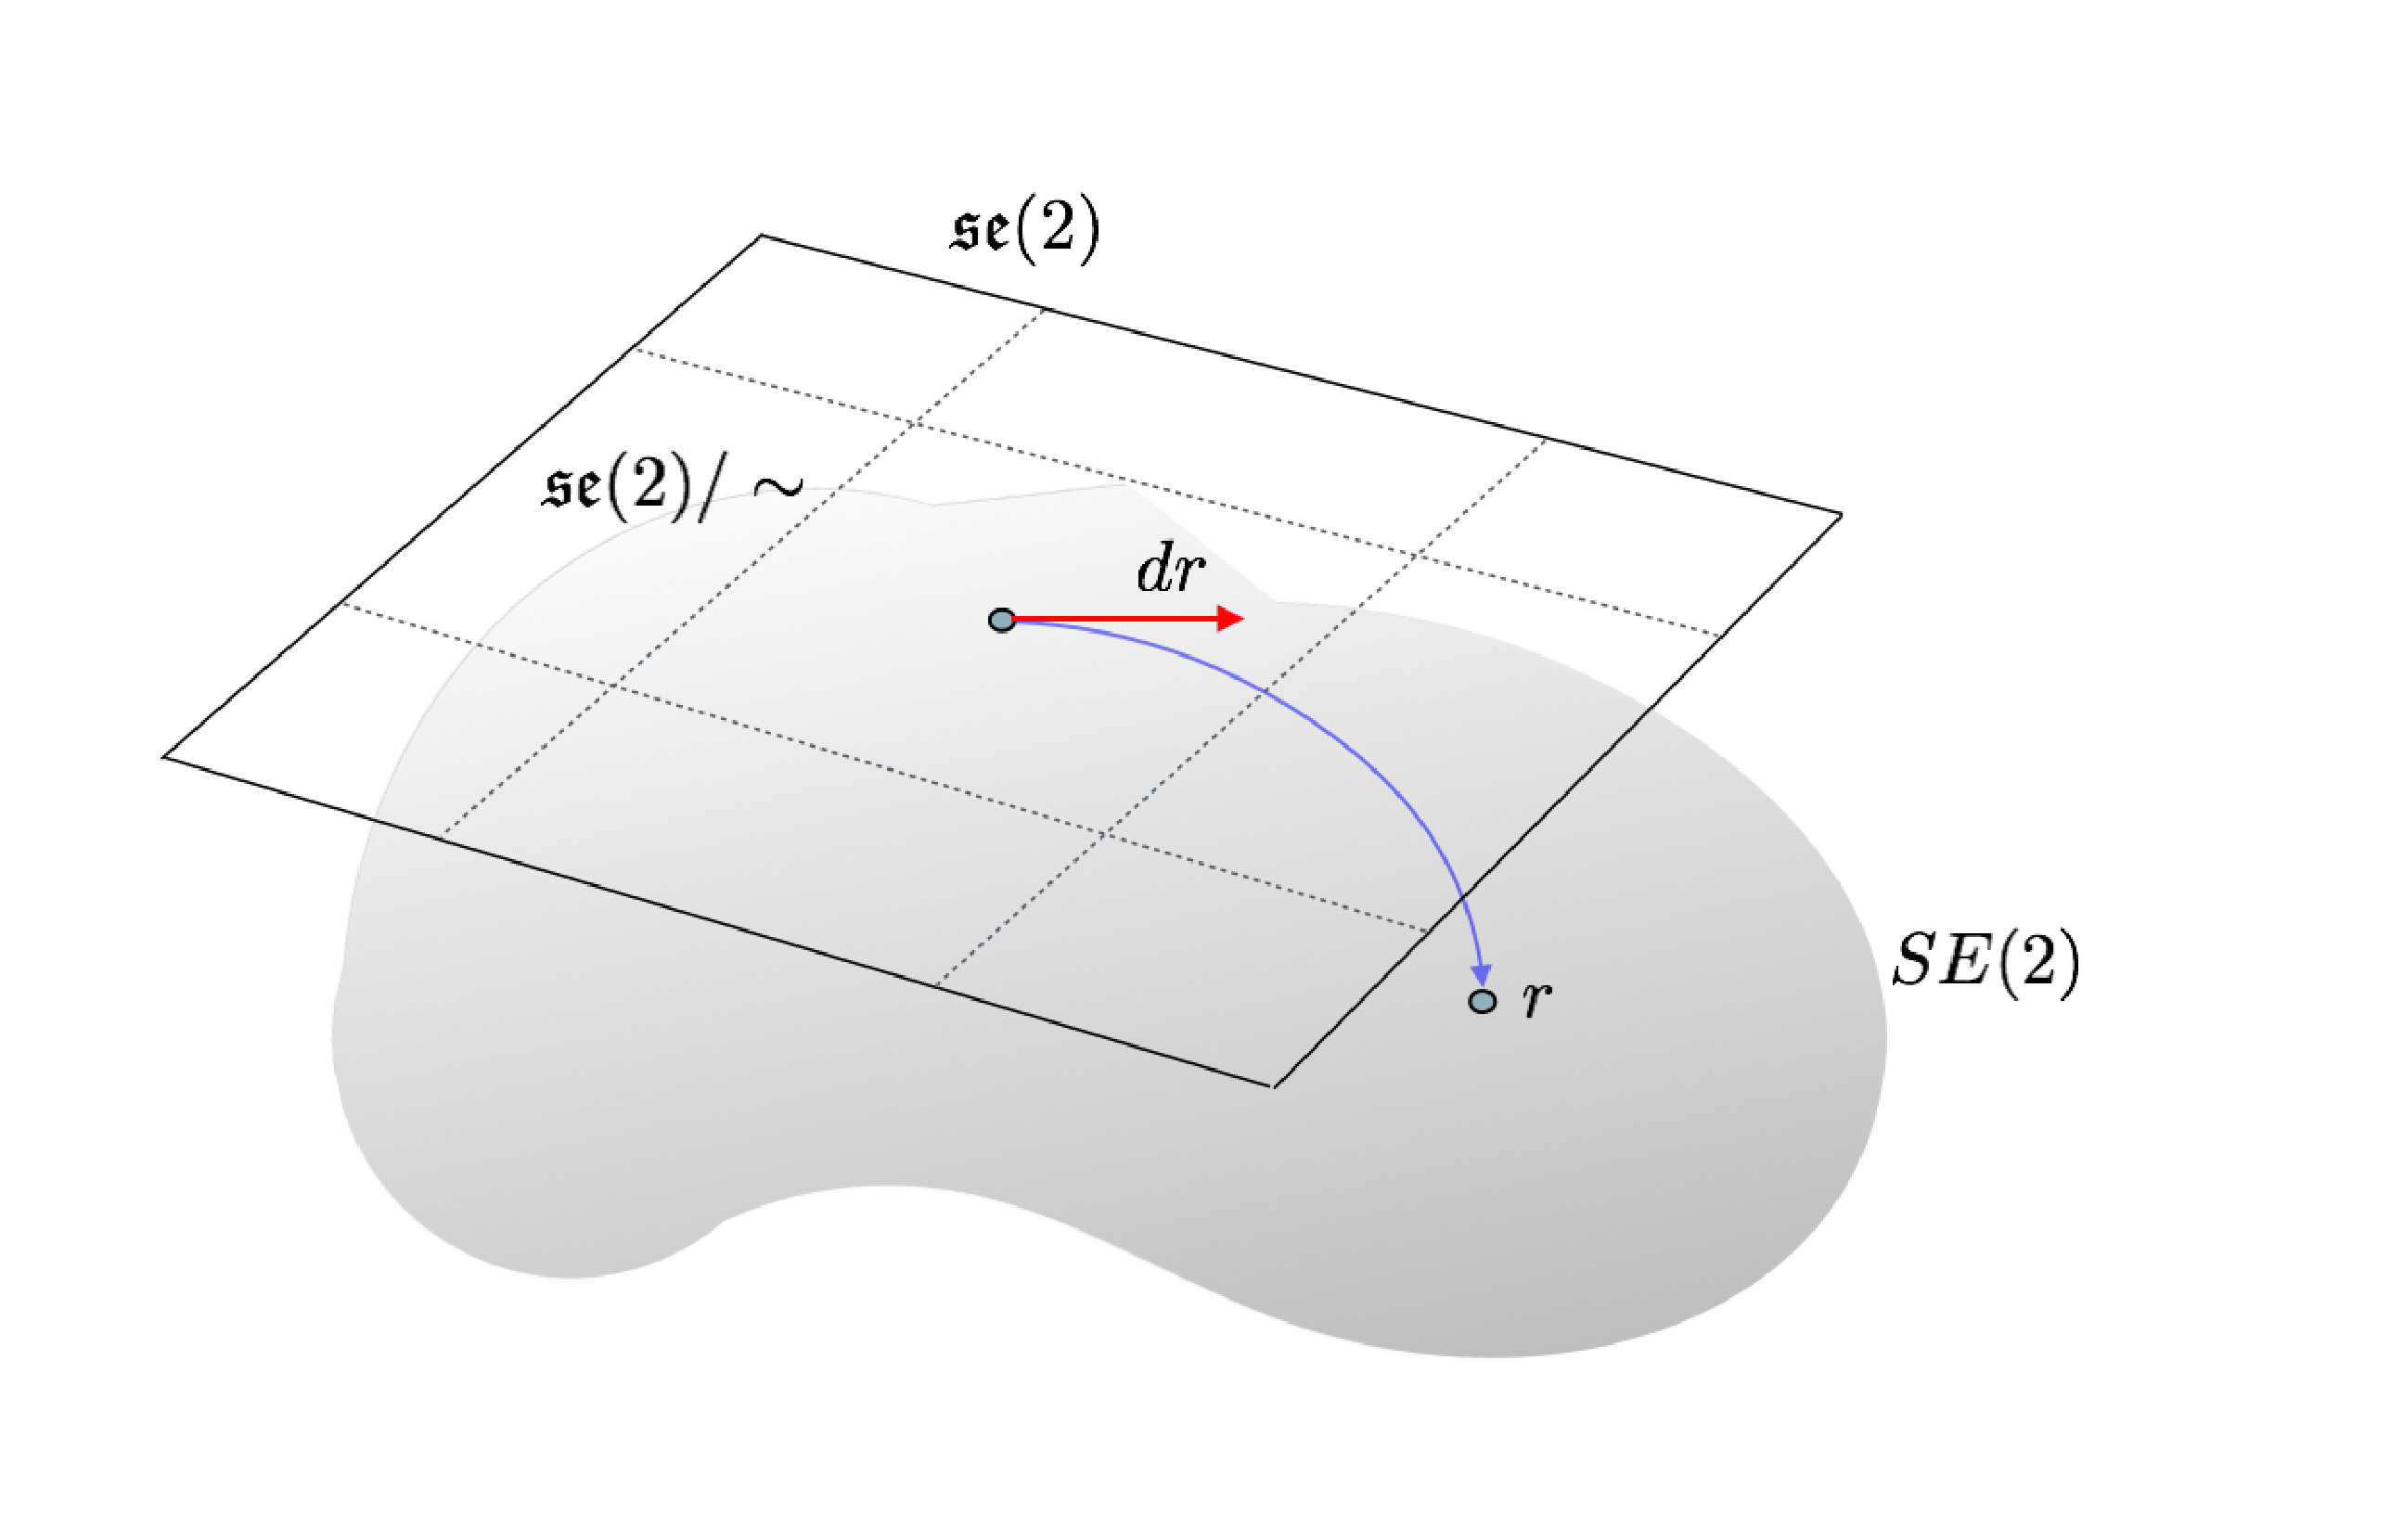
\includegraphics[scale=0.35]{figures/exp_se2.pdf}
		\caption{The Lie algebra $\mathfrak{se}(2)/\sim$ defined as the quotient of the Lie algebra $\mathfrak{se}(2)$ over the equivalence relation $\sim$ is in bijective correspondence with $SE(2)$.}
		\label{fig:exp_se2}
	\end{figure}
	% restriction of the domain.
	\item The map $\exp$ is not well defined as bijection over its whole domain $\mathfrak{se}(2)$. Given two elements $(\theta_0, dt^{x}_0, dt^{y}_0)$ and $(\theta_1, dt^{x}_1, dt^{y}_1)$, they have the same image with $\exp$ function if the two following conditions are both satisfied:
	\begin{enumerate}
		\item[i)] Exists an integer $k$ such that $\theta_0 = \theta_1 + 2k\pi$.
		\item[ii)] the translation $(dt^{x}_0, dt^{y}_0)$ coincides with $(dt^{x}_1, dt^{y}_1)$ up to a factor $\frac{\theta_0}{\theta_1}$, where the angles are considered modulo $2\pi$.
	\end{enumerate}
	To have a bijective correspondence the domain of $\exp$ has to be restricted to a space where if $\exp(\theta_0, dt^{x}_0,dt^{y}_0) = \exp(\theta_1, dt^{x}_1, dt^{y}_1)$ implies  $(\theta_0, dt^{x}_0, dt^{y}_0) = (\theta_1, dt^{x}_1, dt^{y}_1)$.
	It can be easy to prove that the sought space is the quotient of $\mathfrak{se}(2)$ over the equivalence relation $\sim$, defined as 
	\begin{align*}
		(\theta_0, dt^{x}_0, dt^{y}_0 & ) \sim (\theta_1, dt^{x}_1, dt^{y}_1)
		\\
		&\iff_{\text{(by definition)}}
		\\
		\exists k\in\mathbb{Z} \mid \theta_0 = \theta_1 + 2k\pi 
		&~\text{ and }~
		(dt^{x}_0, dt^{y}_0) = \frac{\theta_0}{\theta_1}(dt^{x}_1, dt^{y}_1)
	\end{align*}
	The new algebra defined by the set of equivalence classes of this relation is indicated - with the standard convention, see \cite{artin2011algebra} - with $\mathfrak{se}(2)/\sim$. With this restriction of the domain, the function $\exp$ is a bijection having $\log$ as its inverse.
	What said so far can be summarize in the following commutative diagram:
	
	\[
	\begindc{\commdiag}[40]
	\obj(55,15)[u]{$\mathfrak{se}(2)/\sim $}
	
	%rightside
	\obj(35,30)[se]{$\mathfrak{se}(2)$}
	\obj(35,0)[SE]{$SE(2)$}
	
	% oblique right
	\mor{se}{u}{$\pi$} [\atright,\surjectivearrow]
	\mor{u}{SE}{$\exp$}
	% vertical
	\mor{SE}{se}{$\log$} 
	
	\enddc
	\]

	and with the schematic figure \ref{fig:exp_se2}.
	
\end{enumerate}

% % % % % % % % % % % % % % % % % %
% % % % % % % % % % % % % % % % % % %
\subsection{Computations of Log-composition in $\mathfrak{se}(2)$}
The log-composition of two elements $dr_0 = (\theta_0, dt^{x}_0, dt^{y}_0)$ ans $dr_1 = (\theta_1, dt^{x}_1, dt^{y}_1)$ of $ \mathfrak{se}(2)/\sim$ results
\begin{align}\label{eq:log_composition_se2_closed_form}
& dr_0 \oplus dr_1 =  \log(\exp(dr_0)\circ \exp(dr_1)) 
\end{align}
The approximations of the log-composition using truncated BCH formulas are straightforward:
\begin{align*}
dr_0 \oplus dr_1 &\simeq  BCH^{0}(dr_0,dr_1 ) := dr_0 + dr_1  \\
dr_0 \oplus dr_1 &\simeq BCH^{1}(dr_0,dr_1 ) :=  dr_0 + dr_1 + \frac{1}{2}[dr_0, dr_1] \\
dr_0 \oplus dr_1 &\simeq BCH^{3/2}(dr_{0}, dr_{1}) :=  dr_0 + dr_1 + \frac{1}{2}[dr_0, dr_1] + \frac{1}{12}[dr_0,[dr_0, dr_1]] \\
dr_0 \oplus dr_1 &\simeq BCH^{2}(dr_{0}, dr_{1}) := dr_0 + dr_1 + \frac{1}{2}[dr_0, dr_1] + \frac{1}{12}([dr_0,[dr_0, dr_1]] + [dr_1,[dr_1, dr_0]] )
\end{align*}

To compute the approximation with the Taylor method, and so to compute the equation \ref{eq:taylor} for elements in  $ \mathfrak{se}(2)/\sim$, we observe that the restricted form of the Lie bracket is given by
\begin{align*}
[dr_0, dr_1] &= (0, dR(\theta_0)dt_1 - dR(\theta_1)dt_0)^T \\
& = (0, -\theta_0 dt^{y}_1 + \theta_1 dt^{y}_0 ,  \theta_0 dt^{x}_1 - \theta_1 dt^{x}_0)^T
\end{align*} 
Therefore, the adjoint operator can be written in matrix form as a dual matrix of $dr$:
\begin{align*}
\text{ad}_{dr} = 
\left (
\begin{array} {c c c}
0            &  0        &      0\\
dt^y       &  0        & - \theta \\
- dt^x   & \theta &  0
\end{array}
\right )
\end{align*} 
In fact, when applied to $dr_1$ it results in the Lie bracket:
\begin{align*}
\text{ad}_{dr_0} dr_1= 
\left (
\begin{array} {c c c}
0            &  0        &      0\\
dt^{y}_0       &  0        & - \theta_0 \\
- dt^{x}_0   & \theta_0 &  0
\end{array}
\right )
\left (
\begin{array} {c }
\theta_1   \\
dt^{x}_1   \\
dt^{y}_1 
\end{array}
\right )
=
\left (
\begin{array} {c }
0  \\
-\theta_0 dt^{y}_1+ \theta_1 dt^{y}_0\\ 
 \theta_0 dt^{x}_1- \theta_1 dt^{x}_0
\end{array}
\right )
\end{align*} 
To compute the Taylor approximation proposed in equation \ref{eq:taylor} of the log composition, indicating $dt^{\star} = (dt^{y}, - dt^{x})$ it can be proved easily by induction that
\begin{align*}
\text{ad}_{dr}^{n} 
= 
\left (
\begin{array} {c c}
0            &  0        \\
dt^{\star}      &  dR(\theta)      
\end{array}
\right )^n
=
\left (
\begin{array} {c c}
0            &  0        \\
dR(\theta)^{n-1}dt^{\star}      &  dR(\theta)^{n}      
\end{array}
\right )
\end{align*}
And so the series involved in the equation $\ref{eq:taylor}$ become
\begin{align*}
\sum_{n=0}^{\infty} \frac{B_{n}}{n!} \text{ad}_{dr}^{ n} 
=
\sum_{n=0}^{\infty} \frac{B_{n}}{n!} \left (
\begin{array} {c c}
0            &  0        \\
dR(\theta)^{n-1}dt^{\star}      &  dR(\theta)^{n}      
\end{array}
\right ) 
\end{align*}
We can split it in two part, the rotational part $dR(\theta)^{n}$ and the translational part $dR(\theta)^{n-1}dt^{\star}$. The rotational part, exploiting the nature of Bernoulli numbers and its generative equation, when $\theta \neq 0$ become
\begin{align*}
\sum_{n=0}^{\infty} \frac{B_{n}}{n!} dR(\theta)^{n}  
&=
I + \frac{1}{2}dR(\theta) + \sum_{n=1}^{\infty}\frac{B_{2n}}{2n!} dR(\theta)^{2n}  \\
&=
I + \frac{1}{2}dR(\theta) + (\sum_{n=1}^{\infty}\frac{B_{2n}}{2n!} (i \theta)^{2n})I  \\
&=
\frac{1}{2}dR(\theta) + (\sum_{n=0}^{\infty}\frac{B_{n}}{n!}(i \theta)^{n} - \frac{1}{2} i\theta) I  \\
&=
\frac{1}{2}dR(\theta) + (\frac{i\theta e^{i\theta}}{e^{i\theta} - 1} - \frac{1}{2} i\theta) I  \\
&=
\frac{1}{2}dR(\theta) +  \frac{\theta /2}{\tan(\theta/2)} I  
\end{align*}
where the equation $dR(\theta)^{2n} =  (i \theta)^{2n}I  $. For the translational part we have
\begin{align*}
\sum_{n=1}^{\infty} \frac{B_{n}}{n!} dR(\theta)^{n-1} dt^{\star} 
&=
dR(\theta)^{-1} \Big(\sum_{n=1}^{\infty}\frac{B_{n}}{n!} dR(\theta)^{n}\Big)dt^{\star} \\
&=
dR(\theta)^{-1}  \Big(\sum_{n=0}^{\infty}\frac{B_{n}}{n!} dR(\theta)^{n} - I \Big)dt^{\star}  \\
&=
dR(\theta)^{-1}  \Big(\sum_{n=0}^{\infty} \frac{1}{2}dR(\theta) +  \frac{\theta /2}{\tan(\theta/2)} I  - I \Big) dt^{\star} \\ 
&=
dR(\theta)^{-1}  \Big(\sum_{n=0}^{\infty} \frac{1}{2}dR(\theta) +  \frac{\theta /2}{\tan(\theta/2)} I  - I \Big)dt^{\star} \\
&=
\Big(\frac{1}{2} I + (\frac{\theta /2}{\tan(\theta/2)} - 1)dR(\theta)^{-1}   \Big) dt^{\star}    \\
\end{align*}
Finally the closed form for the Taylor approximation of the log-composition is \cite{vercauteren2014preprint}:
\begin{align}
dr_{0}\oplus dr_{1}
=
dr_{0}
+
\sum_{n=0}^{\infty} \frac{B_{n}}{n!} \text{ad}_{dr_{0}}^{ n} 
dr_{1}
+
\mathcal{O}(dr_{1}^2)
=
dr_{0}
+
\mathbf{J}(dr_{0})
dr_{1}
+
\mathcal{O}(dr_{1}^2)
\end{align}
where 
\begin{align*}
\mathbf{J}(dr_{0})
=
\left (
\begin{array} {c c c}
1            &  0        &      0
\\
-\frac{\theta_0/2 - \tan(\theta_0/2)}{\theta_0\tan(\theta_0/2)}  dt^{x}_0 + \frac{1}{2}dt^{y}_0       
&  \frac{\theta_0 /2}{\tan(\theta_0/2)} 
& - \theta_0/2 
\\
-  \frac{1}{2} dt^{x}_0 -\frac{\theta_0/2 - \tan(\theta_0/2)}{\theta_0\tan(\theta_0/2)} dt^{y}_0       
& \theta_0/2 
&  \frac{\theta_0 /2}{\tan(\theta_0/2)}
\end{array}
\right )
\end{align*}
therefore the corresponding numerical method indicated with the function $\text{Tl}$ as
\begin{align}\label{eq:taylor_se2}
dr_{0}\oplus dr_{1}
\simeq
Tl(dr_{0}, dr_{1})
:=
dr_{0}
+
\mathbf{J}(dr_{0})
dr_{1}
\end{align}

The approximation of the log-composition using parallel transport is a straightforward application of the equation \ref{eq:parallel_transport}: 
\begin{align}\label{eq:parallel_transport_se2}
dr_{0}\oplus dr_{1}
&\simeq
pt(dr_{0}, dr_{1}) 
:=
dr_{0}
+
\exp\big(\frac{dr_{0}}{2}\big)   
\exp(dr_{1}) 
\exp\big(-\frac{dr_{0}}{2}\big)
-
I
\end{align}
where the composition in the Lie group coincides with the product of matrix in the bigger algebra $GL(3)$ that contains both the Lie group $SE(2)$ and the Lie algebra $\mathfrak{se}(2)$.


% % % % % % % % % % % % % % % % % % % % % % % % % % % % % % % % % % % %
% % % % % % % % % % % % % % % % % % % % % % % % % % % % % % % % % % % %
% % % % % % % % % % % % % % % % % % % % % % % % % % % % % % % % % % % %
% % % % % % % % % % % % % % % % % % % % % % % % % % % % % % % % % % % %
\section{The Lie group of Diffeomorphisms}\label{se:svf}


The passage from the finite to the infinite dimensional case is not free of deceptions. We will investigate in the next two subsections, \ref{subse:local_isomorphisms} and \ref{subse:bigger_algebra} ,the following facts that are true matrices but not for diffeomorphisms:
\begin{enumerate}
	\item Lie logarithm and Lie exponential are local isomorphisms.
	\item $SE(2)$ and $\mathfrak{se}(2)$ are subset of a bigger algebra, where all of the operations are compatible.
\end{enumerate}
These will be analyzed in the next two sections, but to avoid ambiguities, we first need to write down some definitions and facts.

\begin{figure}[!ht]
	\hspace{-1.5cm}
	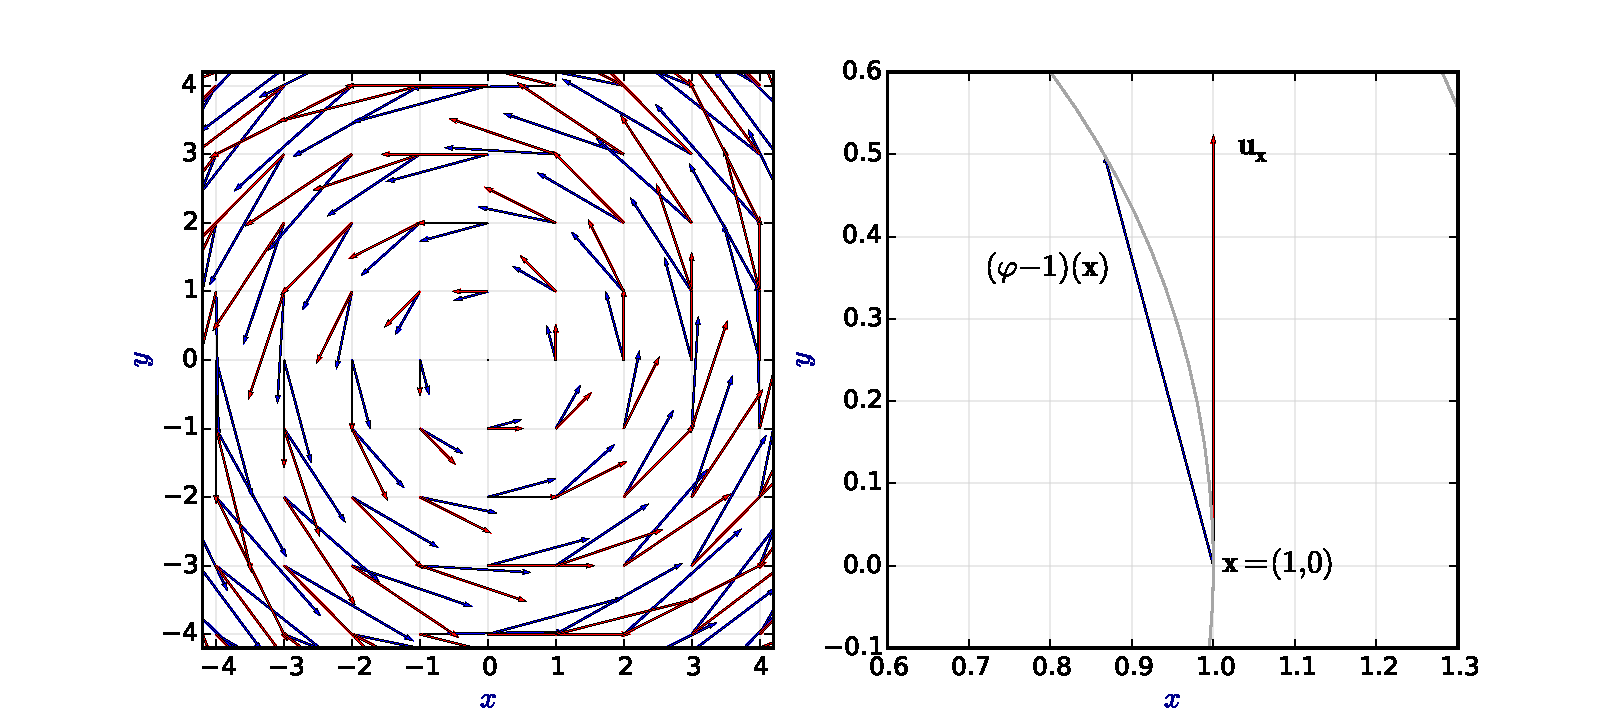
\includegraphics[scale=0.6]{figures/se2_circular_vector_field.pdf}
	\caption{the displacement field and the tangent vector field for the transformation $\varphi$ defined as a rotation of $\pi / 6$ around the origin. When $\varphi$ is subtracted by the identity function, become an element of the algebra of the velocity vector fields $\text{Vect}(\Omega)$.}
	\label{fig:se2_circular_vector_field}
\end{figure}

We define the set of \emph{deformations}, the set of continuous functions from $\Omega$ to $\Omega$, compact subset of $\mathbb{R}^d$. If a deformation is invertible with continuous inverse, then it is called \emph{homeomorphism}; the set of homeomorphisms forms a group, indicated with $\text{Hom}(\Omega)$, with the operation of function composition. If an homeomorphism is differentiable and has differentiable inverse then it is called \emph{diffeomorphism}. Again the set of diffeomorphisms forms a group, indicated with $\text{Diff}(\Omega)$.

A \emph{velocity vector field} over $\Omega$ is a differentiable function that at each point of $\Omega$, associates a vector of $\mathbb{R}^d$; the set of velocity vector fields, indicated with $\text{Vect}(\Omega)$ forms a vector space, and considering the Lie bracket defined by the directional derivative
we obtain that $\text{Vect}(\Omega)$ forms a Lie algebra\footnote{
	Some books invert the signs of the operation (see the Kirillow's remarks \cite{kirillov2008introduction} pag. 27); this choice do not have any impact in the study of the algebraic structure, but it does have an impact on the numerical results when the Lie brackets are implemented for numerical computations. At the moment the sign that defines the Lie bracket is chosen on the base of the obtained results.
}.
If $\{\frac{\partial}{\partial x_{i}}\}_{i=1}^{d}$ is a local coordinates system over $\Omega$, $\mathbf{u}=a^{i} \frac{\partial}{\partial x_{i}}$ and $\mathbf{v}=b^{i} \frac{\partial}{\partial x_{i}}$ are two elements of  $\text{Vect}(\Omega)$ written using the Einstein summation convention, the Lie bracket can be expressed using the Jacobian:
\begin{align*}
[\mathbf{u}, \mathbf{v}] &= 
a^{i} \frac{\partial}{\partial x_{i}}\big( b^{j} \frac{\partial}{\partial x_{j}} \big)
-
b^{i} \frac{\partial}{\partial x_{i}}\big( a^{j} \frac{\partial}{\partial x_{j}} \big) \\
&=
a^{i} \frac{\partial b_{j}}{\partial x_{i}}\frac{\partial}{\partial x_{j}}  
+ 
a^{i}b^{j}\frac{\partial^{2}}{\partial x_{i}x_{j}}
- 
b^{j} \frac{\partial a^{i}}{\partial x^{j}}\frac{\partial}{\partial x_{i}} 
-
b^{j}a^{i}\frac{\partial^{2}}{\partial x_{j}x_{i}} \\
&=
a^{i} \frac{\partial b_{j}}{\partial x_{i}}\frac{\partial}{\partial x_{j}}
-
b^{j} \frac{\partial a^{i}}{\partial x^{j}}\frac{\partial}{\partial x_{i}} 
= J_{\mathbf{v}}\mathbf{u} - J_{\mathbf{u}}\mathbf{v}
\end{align*}

% here the two doors
It was proved that the Lie algebra of the Lie group of diffeomorphisms $\text{Diff}(\Omega)$ is $\text{Vect}(\Omega)$ (\cite{milnor1982infinite}, \cite{ovsienko1992integrals}). 
Therefore a single vector in the Lie algebra $\text{Vect}(\Omega)$ (represented by one red arrow in figure \ref{fig:composition}) is a vector field defined over $\Omega$ (represented by the set of red arrows in figure \ref{fig:se2_circular_vector_field}). We would expect that, vice versa, to a single diffeomorphism in the Lie group corresponds a single vector of the Lie algebra. This is not the case, since Lie logarithm and Lie exponential are not local isomorphisms on the whole domain.

% % % % % % % % % % % % % % % % % % % % % % % % % % % % % % % % % % % %
% % % % % % % % % % % % % % % % % % % % % % % % % % % % % % % % % % % %
\subsection{Local isomorphisms for a subset of Diffeomorphisms: one-parameter subgroup and stationary velocity fields}\label{subse:local_isomorphisms}

In the case of matrices, the exponential map is a local isomorphisms: it is always possible to find an open neighbor of $\mathbf{0}$ in the Lie algebra and an open neighbor of the identity element in the Lie group (in the same topology induced by the metric inherited by the bigger algebra), such that the exponential map is defined and invertible.

In the infinite dimensional case there are diffeomorphisms arbitrarily close to the identity that are not embedded to any one-parameter subgroups, therefore the exponential map is not a local isomorphism (see the counterexample in \cite{milnor1984remarks}, pag. 1017 or the definition of Koppel-diffeomorphisms \cite{grabowski1988free} pag. 115).

% subset of diff in which we are interested: the one that can be parmetrized by tangent vector fields
Since for medical image registration we are interested only in the diffeomorphisms that can be parametrized by tangent vector fields, this feature is worthed to be investigated, but it requires some definitions.

% two kinds of vector fields. TVVF SVF. A continuous way to produce diffeomorphims
If $\varphi$ is a one-parameter subgroup on the manifold $\text{\emph{Diff}}(\Omega)$, then its derivative satisfies the \emph{stationary} (or homogeneous) ordinary differential equation:
\begin{align}\label{eq:generating_ODE_svf}
\frac{d\varphi(t)}{dt} = V_{\varphi(t)}
\end{align}
Where the stationary vector field $V_{\varphi(t)}$ defined over $\Omega$ is an element of the Lie algebra of $\mathcal{V}(\Omega)$ called \emph{stationary velocity field} or SVF. In fact
\begin{align*}
\frac{d\varphi(t)}{dt} 
= 
\lim_{\epsilon \rightarrow 0} \frac{\varphi(t +\epsilon)}{\epsilon} 
=
\lim_{\epsilon \rightarrow 0} \frac{\varphi(\epsilon) \varphi(t)}{\epsilon} 
=
V_{\varphi(t)}
\end{align*} 

Vice versa, given an SVF, thanks to Cauchy theorem exists always a unique solution $\varphi$ to the ODE \ref{eq:generating_ODE_svf}, given the initial condition $\varphi(0) = 1$, that satisfies the property of one-parameter subgroup.

We indicate with $\text{\emph{Diff}}^{1}(\Omega)$ the \emph{set of diffeomorphisms embedded in a one parameter subgroup}, i.e. the solutions of \ref{eq:generating_ODE_svf}. We notice that $\text{\emph{Diff}}^{1}(\Omega)$ does not form a group. In fact if $\varphi$ and $\psi$ are in $\text{\emph{Diff}}^{1}(\Omega)$ and satisfy respectively $\frac{d\varphi_1(t)}{dt} = U_{\varphi_1(t)}$ and $\frac{d\varphi_2(t)}{dt} = V_{\varphi_2(t)}$, then their composition $\varphi_1\circ\varphi_2$ does not satisfy any stationary ordinary differential equation. 
To have closure for the composition of one parameter subgroup, we have to extend our attention to non stationary (or non homogeneous) ordinary differential equation of the form:
\begin{align}\label{eq:generating_ODE_tvvf}
\frac{d\psi(t)}{dt} = W_{(t, \psi(t))}
\end{align}
Where $W_{(t, \psi(t))}$ is a non-stationary vector field, called here time varying vector field, or TVVF. If compared with to the SVF, it does not depends only on the spatial position $\mathbf{x}$ but there is also a temporal dependency. 

Think for example to a satellite orbiting around the globe: it is subject to the earth's vector field in respect to which it is constant for a fixed position, and to the lunar vector field that it is not fixed but varies in respect to the time. Conventionally the temporal domain $T$ contains the origin and formally we can write:
\begin{align*}
W : T\times \Omega & \longrightarrow  \mathbb{R}^d \\
t, \psi(t) &\longmapsto  W_{(t, \psi(t))}
\end{align*}
for $\psi$ diffeomorphism (or in the previous example, position of the satellite at time $t$) that when applied to a point of $\Omega$ is indicated with $\varphi(t,\mathbf{x})$ or $\psi^{(t)}(\mathbf{x})$.

A crucial observation for our purpose is that non-autonomous ODE are particular cases of autonomous one. Writing the diffeomorphism $\psi(t)$ applied to $\mathbf{x}$ in local coordinates as 
\begin{align*}
\psi^{(t)}(\mathbf{x}) = (\psi_1^{(t)}(\mathbf{x}), \psi_2^{(t)}(\mathbf{x}), \dots ,\psi_d^{(t)}(\mathbf{x})) \in \mathbb{R}^{d}
\end{align*}
Defining a new function $\psi_0^{(t)}(\mathbf{x}) = t_0 + t$ for all $\mathbf{x} \in \Omega$, we can obtain then the new diffeomorphism $\tilde{\psi}^{(t)}$ that in local coordinates is expressed as 
\begin{align*}
\tilde{\psi}^{(t)}(\mathbf{x}) = (\psi_0^{(t)}(\mathbf{x}), \psi_1^{(t)}(\mathbf{x}), \psi_2^{(t)}(\mathbf{x}), \dots ,\psi_d^{(t)}(\mathbf{x})) \in T\times \mathbb{R}^{d}
\end{align*}
that reduces the ODE \ref{eq:generating_ODE_tvvf} to an ODE of the form \ref{eq:generating_ODE_svf}. In the example of satellite, is like considering the temporal dimension as an additional dimension of the space. The vector that influence the satellite is an SVF for every point in the domain of space-time. 

It follows that tationary ODE and non-stationary ODE have solutions that belong to $\text{\emph{Diff}}^{1}(\Omega)$ and $\text{\emph{Diff}}^{1}(T\times \Omega)$ respectively. For each instant of time the solution of non-stationary ODE, are embedded in the set of one-parameter subgroup of $\text{\emph{Diff}}(\Omega)$, but for two different instant of time, the solution can belongs to two different elements in the one parameter subgroups. 

In conclusion, we have that there in the case of diffeomorphisms $\exp$ is not a local isomorphism, unless we do not restrict the group of diffeomorphisms to the one embedded in a one parameter subgroup $\text{\emph{Diff}}^{1}(T\times \Omega)$. In addition the set of diffeomoerphisms restricted to the one that solves the equation \ref{eq:generating_ODE_svf} does not form any group with the composition. This happen only if we extend to the solution of the non stationary ODE \ref{eq:generating_ODE_tvvf}, and therefore to TVVF. In addition, indicating with $\text{SVF}$ the set of stationary velocity fields and with $\text{TVVF}$ the set of time varying velocity fields, we have that
\begin{align*}
\text{\emph{Diff}}^{1}(\Omega) &= \exp(\text{SVF}) = \exp(\text{TVVF})
\end{align*}
but to a given SVF exists only one one-parameter subgroup $\varphi$ that satisfies the ODE \ref{eq:generating_ODE_svf}. The same thing does not necessarily happens for the TVVF.

In the LDDMM framework \cite{beg2005computing} TVVFs are initially considered, while with the paper of Arsigny \cite{arsigny2006log}, and in subsequent works, the attention has been restricted to SVF, in order to be able to use the scaling and squaring and the inverse scaling and squaring algorithms for the numerical computation of the Lie exponential and the Lie logarithm. In fact the scaling and squaring method, as every numerical method based on the phase flow \cite{ying2006phase}, works only under the assumption that the transformation belongs to the same one-parameter subgroup.


% % % % % % % % % % % % % % % % % % % % % % % % % % % % % % % % % % % %
% % % % % % % % % % % % % % % % % % % % % % % % % % % % % % % % % % % %
\subsection{A bigger algebra for the group of Diffeomorphisms}\label{subse:bigger_algebra}
As well as for any matrix Lie group, both the group $SE(2)$ and the algebra $\mathfrak{se}(2)$ are subset of the same bigger algebra of matrices in the general linear group $GL(3,\mathbb{R})$. The product of the algebra coincides with the composition of the group and thanks to the linearity, scalar product is compatible both with the product and the composition.

The existence of a bigger algebra is not important only in the research of an elegant structure: the power series expansions of the exponential (\ref{eq:exp_as_inf_sum}) and the logarithm (\ref{eq:log_as_inf_sum}) as well as expressions like (\ref{eq:prop_matrix_diff_log}) and (\ref{eq:prop_matrix_lim}) would be meaningless without the possibility of expressing the sum of two elements of a multiplicative group. Moreover, if the bigger algebra that contains both Lie group and Lie algebra exists, a unique norm in this space can be defined and utilized to compare elements in the both subspaces.

In the case of diffeomorphism of the compact subset $\Omega$ of $\mathbb{R}^d$, we can identify a bigger vector space that contains both Lie group and Lie algebra, but it is less straightforward than in the case of matrices, and for this aim it is necessarily to have some definitions at hand.

\begin{figure}[!ht]
	\centering
	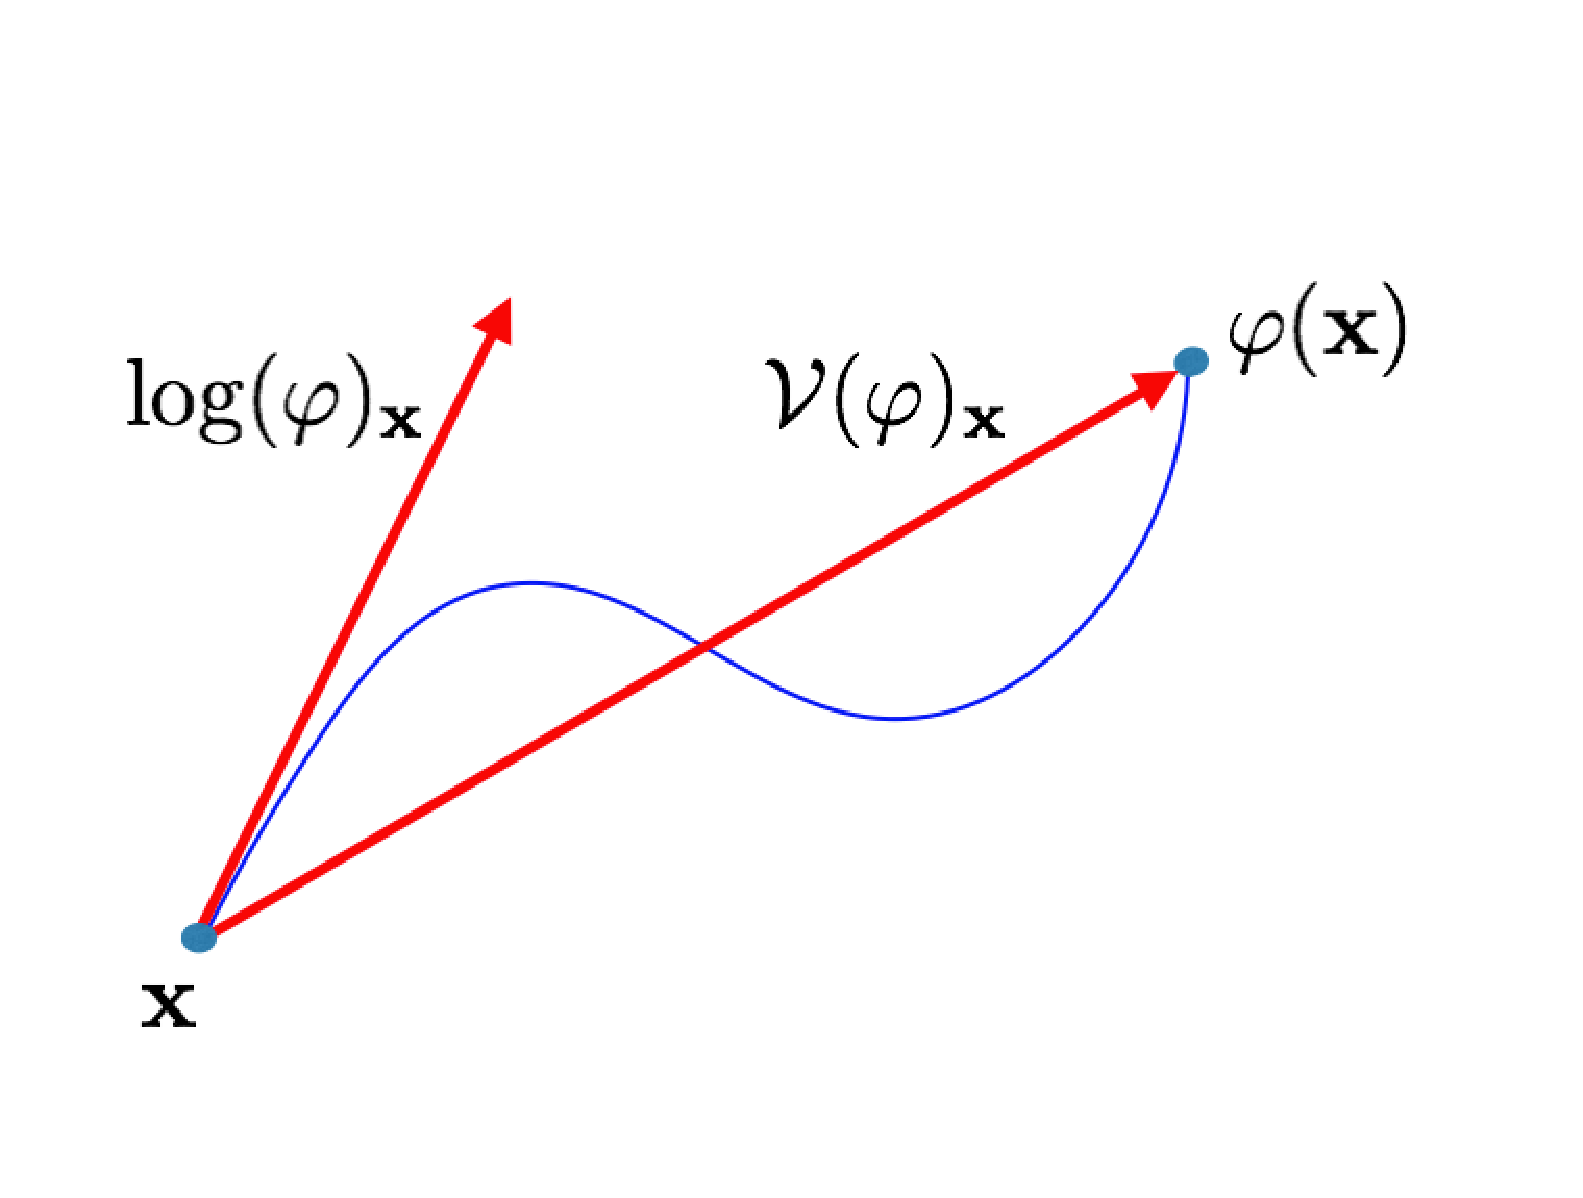
\includegraphics[scale=0.25]{figures/exp_versus_v.pdf}
	\caption{for small deformations, the displacement field $\log(\varphi)$ and the tangent field $\mathcal{V}(\varphi)$, computed at the point $\mathbf{x}$ of $\Omega$, are close to each others.}
	\label{fig:exp_versus_v}
\end{figure}

There are two ways to associate a diffeomorphisms $\varphi$ to a velocity vector field. The first one is elementary but fundamental in this context: it consists in subtracting to $\varphi$ the identity function $1$. If $\mathbf{x}$ is in $\Omega$ and $\varphi(\mathbf{x})$ is the new point after the transformation, then the associated velocity vector field, called here \emph{displacement field of} $\varphi$, is the function that at the point $\mathbf{x}$ associate the vector defined as the difference $\varphi(\mathbf{x}) - \mathbf{x}$. To recover the deformation from a velocity field $\mathbf{u}$ is enough to add the identity; in this case we have the \emph{deformation of} $\mathbf{u}$. We indicate this operation of adding and subtracting the identity with the function $\mathcal{V}$:
\begin{align*}
\mathcal{V}(\varphi) = \varphi - 1 
\qquad \qquad
\mathcal{V}^{-1}(\mathbf{u}) = \mathbf{u} + 1 
\end{align*}
We can see that displacement fields of diffeomorphisms are elements of $\mathcal{V}(\Omega)$, that is the analogous of the bigger algebra that contains Lie group and Lie algebra in the case of matrices. We can observe that this operation of subtracting the identity to the deformation has already been used implicitly in the power series expansion of the Lie logarithm for matrices, see equation \ref{eq:log_as_inf_sum}.

The second way to associate a velocity vector field to $\varphi$ is with the Lie logarithm defined in the chapter \ref{ch:tools}. It is interesting to notice that when $\mathbf{u}$ is small then $\mathcal{V}^{-1}$ and $\exp$ are closed to each other and $\mathcal{V}^{-1}$ can be considered a good approximation of $\exp$ (see figure \ref{fig:exp_versus_v}). The very same happens for matrices, as noticed in equations (\ref{eq:small_rotation_matrices_approx}).

At this point it is important to notice that, while a displacement field of $\varphi$ can always be defined, the exponential map it is not defined for any diffeomorphism. This is the second remarkably difference between the matrix Lie group and the Lie group of diffeomorphisms that will be investigated in the next section.



% % % % % % % % % % % % % % % % % %
% % % % % % % % % % % % % % % % % % %
\subsection{A Norm for the Elements in the one-parameter subgroup}\label{subse:norm}
A metric between tangent vector fields of $\Omega$ can be defined as 
\begin{align}\label{def:metric_two_svf}
d(\mathbf{u}, \mathbf{v}) 
= 
\Big( \int_{\Omega} \euclideanMetric{\mathbf{u} - \mathbf{v}}_{L^2}^{2} d\mathbf{x} \Big)^{1/2}
\end{align} 
that naturally induces a metric on the Lie algebra.

The Lie group $\text{\emph{Diff}}^{1}(\Omega)$ do not possess any norm, but the corresponding displacement fields defined by $\mathcal{V}$, as tangent vector fields does. Given two diffeomorphisms $\varphi_0$ and $\varphi_1$ we have
\begin{align}\label{def:metric_two_displacement_field}
d^{1}(\varphi_0,\varphi_1) 
= 
\Big( \int_{\Omega} \euclideanMetric{\mathcal{V}(\varphi_0) - \mathcal{V}(\varphi_1)}_{L^2}^{2} d\mathbf{x} \Big)^{1/2}
\end{align} 
Despite the limitation that Lie algebra and Lie group of diffeomorphisms are not subset of the same bigger algebra, we can nevertheless consider a function that measure the best approximation of metric we can have for $\text{\emph{Diff}}^{1}(\Omega)$ and SVF:
\begin{align}\label{def:metric_one_svf_one_displacement_field}
d^{m}(\mathbf{u},\varphi) 
= 
\Big(\int_{\Omega} \euclideanMetric{\mathbf{u} - \mathcal{V}(\varphi)}_{L^2}^{2} d\mathbf{x} \Big)^{1/2}
\end{align} 
The next section is about the parametrization of SVF in the applications, and it is followed by the one that presents the numerical methods for the log-composition when applied to SVF.

% % % % % % % % % % % % % % % % % %
% % % % % % % % % % % % % % % % % % %
\subsection{Parametrization of SVF: Grids and Discretized Vector Fields}\label{se:parametrization_SVF}

Even if images are discrete elements, the underpinning model of the transformations is based on the continuous. There are several motivations that led to this choice: as underlined by \cite{szeliski1994image}, the most important is that images are discrete measurement of the continuous property of an object. Therefore it is reasonable have a model as close as possible to the continuous object rather than to a set of discrete measurements. 
Certainly it is important to keep in mind the fact that the continuous approximation is obtained - in a non unique way - from the discretized image with an interpolation scheme. This imply that, for example if the distance between two separate objects is less than the size of a voxel, in continuous approximation based on the discretized image the two object will be not anymore separated. 

Also transformations between images are discretized vector fields, where each vector is applied to an element of a grid. These transformations can only be considered as a model of the group of diffeomorphisms (a model of a model, in image registration!) and reflects only partially the continuous property of the original transformation.
On the other side the possibility of working with discretized elements means working with something that can be managed by computers.

As in many implementation, the data structure utilized to store images, as well as displacement fields are 5-dimensional matrices
\begin{align}\label{eq:basic_data_structure}
M = M(x_i,y_j,z_k,t,d) \qquad (i,j,k)\in L , ~~ t \in T  ~~ d = 1,2,3
\end{align}
where $(x_i,y_j,z_k)$ are discrete position of a lattice $L$ in the domain of the images, $t$ is the time parameter in a discretized domain $T$ and $d$ is index of the coordinate axis. So, the discretized \emph{tangent vector} $\mathbf{v}_{\tau}(x_i,y_j,z_k)$ at time $t$, has coordinates defined by
\begin{align*}
\mathbf{v}_{t}(x_i,y_j,z_k) = (M(x_i,y_j,z_k,t ,1), M(x_i,y_j,z_k,t,2), M(x_i,y_j,z_k,t ,3))
\end{align*}


% % % % % % % % % % % % % % % % % %
% % % % % % % % % % % % % % % % % % %
\subsection{Computations of Log-composition for SVF}\label{se:log_composition_SVF}
A closed-form for the Taylor Expansion method \ref{se:taylor_expansion} to compute the log-composition with elements in $\text{\emph{Diff}}^{1}(\Omega)$ is not known. We will therefore compare the truncated BCH formula with the parallel transport method \ref{se:parallel_transport}. 
The Lie bracket that appears of SVF in the truncated $BCH$ of degree $0,1,1.5$ and $2$, are computed using the Jacobian matrix $J$:
\begin{align}
[\mathbf{u},\mathbf{v}] :=J_{u}\mathbf{v} - J_{u}\mathbf{v}  
\qquad
\forall \mathbf{u},\mathbf{v} \in \mathfrak{g}
\end{align}
as a consequence of its definition (see \cite{lee2012introduction}).
It has been shown that this definition is uniquely defined as action on the space of $\mathbb{C}^{\infty}$ function on the same domain and it satisfies the axioms of Lie bracket of a Lie algebra.\\

Therefore the truncated approximation of the BCH formula presented in the equation \ref{eq:bch_definition} become:
\begin{align*}
BCH^{0}(\mathbf{u},\mathbf{v}) &= \mathbf{u} + \mathbf{v} \\
BCH^{1}(\mathbf{u},\mathbf{v}) &=  \mathbf{u} + \mathbf{v} + \frac{1}{2}(J_{\mathbf{u}}\mathbf{v} - J_{\mathbf{u}}\mathbf{v})\\
BCH^{3/2}(\mathbf{u},\mathbf{v}) 
&=  
\mathbf{u} + \mathbf{v} + \frac{1}{2}(J_{u}\mathbf{v} - J_{u}\mathbf{v}) + 
\frac{1}{12}\big( 
2 J_{\mathbf{u}} J_{\mathbf{u}}\mathbf{v} +2 J_{\mathbf{u}} J_{\mathbf{v}}\mathbf{u}
- 
J_{(J_{\mathbf{u}}\mathbf{v} - J_{\mathbf{u}}\mathbf{v})}\mathbf{u} 
\big) 
\\
BCH^{2}(\mathbf{u},\mathbf{v}) 
&=  
\mathbf{u} + \mathbf{v} + \frac{1}{2}(J_{u}\mathbf{v} - J_{u}\mathbf{v}) 
\\
&+ 
\frac{1}{12}\big( 
2 J_{\mathbf{u}} J_{\mathbf{u}}\mathbf{v} +2 J_{\mathbf{u}} J_{\mathbf{v}}\mathbf{u}
- 
J_{(J_{\mathbf{u}}\mathbf{v} - J_{\mathbf{u}}\mathbf{v})}\mathbf{u} 
+
2 J_{\mathbf{v}} J_{\mathbf{v}}\mathbf{u} +2 J_{\mathbf{v}} J_{\mathbf{u}}\mathbf{v}
- 
J_{(J_{\mathbf{v}}\mathbf{u} - J_{\mathbf{v}}\mathbf{u})}\mathbf{v} 
\big) 
\end{align*}
Lie brackets of SVF can become extremely small, in particular, as we will see in the last chapter, when the standard deviation of the Gaussian filter that generates the fields is small. \\
Whether it is not known how to apply Taylor method presented in \ref{se:taylor_expansion} for the SVF, the parallel transport method for the computation of the log-composition follows directly from equation  \ref{eq:parallel_transport}:
\begin{align*}
\mathbf{u}_0\oplus \mathbf{u}_1
&\simeq
\mathbf{u}_0 
+
\exp_{e}\big(\frac{\mathbf{u}_0}{2}\big)   
\circ  \exp_{e}(\mathbf{u}_1) 
\circ \exp_{e}\big(-\frac{\mathbf{u}_0}{2}\big)
-
e
\end{align*}
Here the exponential function can be computed with several algorithms (scaling and squaring, forward Euler, composition method, Taylor expansion, see \cite{bossa2008algorithms} for a comparison of their performances). Following the original setting of the Log-euclidean metric proposed in \cite{arsigny2006log} we use the scaling and squaring, keeping in mind that this choice impact on the results.









\chapter{Log-composition to Compute the Lie Logarithm}\label{ch:log_algorithm}

\begin{flushright}
	I think you might do something better with the time \\ than wasting it in asking riddles that have no answers. \\ -\emph{Alice in Wonderland.}
\end{flushright}

\vspace{0.5 cm}

\noindent
The \emph{logarithm computation problem} can be stated as follows:
\begin{center}
\emph{
	Given $p$ in a Lie group $\mathbb{G}$, \\ 
	what is the element $\mathbf{u}$ in its Lie algebra $\mathfrak{g}$ \\
	such that $\exp(\mathbf{u}) = p$ ?  
}
\end{center}
There are several numerical methods to compute the approximation of the problem's solution. Arsigny, who first pointed the applications of the Lie logarithm in medical image registration in \cite{Arsigny:MRM:06} and \cite{arsigny2006bi}, proposed the Inverse scaling and squaring (see also \cite{ying2006phase}). In this chapter we investigate other numerical iterative algorithms for the computation of the Lie logarithm, called here \emph{logarithm computation algorithm}; they modifications of the algorithm presented in \cite{Bossa:08} that is based on the BCH formula, and so on the log-composition. Each of the numerical method to compute the log-composition become naturally a numerical method for the computation of the logarithm computation algorithm.\\
The first step toward this direction is to introduce the space of the approximations of a Lie algebra and a the Lie group.


% % % % % % % % % % % % % % % % % % % % % % % % % % % % % % % % % % % % % %
% % 
% % % % % % % % % % % % % % % % % % % % % % % % % % % % % % % % % % % % % % 
\section{Spaces of Approximations}\label{se:space_of_approximation}

\noindent
As seen in section \ref{se:rigid_body_transformations} and \ref{se:svf}, if the element $\mathbf{u}$ of $\mathfrak{se}(2)$ or SVF is small enough we can approximate $\exp(\mathbf{u})$ with $e + \mathbf{u}$. Aim of this section is to investigate these approximations aimed to compute the logarithm.  \\
Let $C_\mathfrak{g}$ and $C_\mathbb{G}$ the internal cut locus of a Lie algebra and a Lie group $\mathfrak{g}$ and $\mathbb{G}$ (the subset where the exponential map is well defined).
We define two approximating functions:
\begin{align*}
\text{app} : C_\mathfrak{g} & \longrightarrow  C_\mathfrak{g}^{\sim}    \\
\mathbf{u} &\longmapsto \exp(\mathbf{u}) - e
\end{align*}
\begin{align*}
\text{App} : C_\mathbb{G} & \longrightarrow  C_\mathbb{G}^{\sim}   \\
\exp(\mathbf{u}) &\longmapsto e + \mathbf{u}
\end{align*}
Where $C_\mathfrak{g} ^{\sim}$ is the space of approximations of elements of $C_\mathfrak{g} $, and $C_\mathbb{G}^{\sim} $ is the space of approximations of elements in $C_\mathbb{G}$, defined as
\begin{align*}
C_\mathfrak{g} ^{\sim} & := \{ \exp(\mathbf{u}) - e \mid \mathbf{u}\in C_\mathfrak{g}\} \cup C_\mathfrak{g} \\
C_\mathbb{G}^{\sim}  & := \{ e + \mathbf{u} \mid \mathbf{u}\in C_\mathbb{G}\} \cup C_\mathbb{G} \\
\end{align*}
In general $C_\mathfrak{g}^{\sim} \neq C_\mathfrak{g}$ and $C_\mathbb{G}^{\sim} \neq C_\mathbb{G}$, but in the considered cases of $\mathfrak{se}(2)$ and SVF, when $\mathbf{u}$ is \emph{small enough}
it follows that $\exp(\mathbf{u}) - e \in C_\mathfrak{g} $ and $e + \mathbf{u}\in C_\mathbb{G}$. Therefore the elements of $C_\mathfrak{g}^{\sim} $ are compatible with all of the operations of the internal cut locus of the Lie algebra $C_\mathfrak{g}$ and the elements of $C_\mathbb{G}^{\sim}$ are compatible with all of the operations of Lie group $\mathbb{G}$.\\
Lets examine what does \emph{small enough} means in these two cases:
\begin{enumerate}
	\item[$\mathfrak{se}(2)$ -] Since $\mathfrak{se}(2)$ and $SE(2)$ are subset of the bigger algebra $SE(2)$ then exp and log can be defined as infinite series. From 
	\begin{align*}
	\exp(\mathbf{u}) = I + \mathbf{u} + O(\mathbf{u}^2) 
	\end{align*}
	It follows that $\text{app}(\mathbf{u}) - \mathbf{u} = O(\mathbf{u}^2)$. Thus for all $\mathbf{u}$ in the internal cut locus smaller than $\delta$ for any norm, exists $M(\delta)$ such that
	\begin{align*}
	\euclideanMetric{\text{app}(\mathbf{u}) - \mathbf{u} } < M(\delta) \euclideanMetric{\mathbf{u}^2}
	\end{align*}
	\item[SVF -] In case of SVF we do not have any Taylor series and big-O notation available but, according to the proposition 8.6 at page 163 of \cite{younes2010shapes}, if $\mathbf{u}$ is, for any norm, smaller than $\epsilon<1/C$, where $C$ is the Lipschitz constant in the same norm, then $1 + \mathbf{u}$ is a diffeomorphism. With this condition holds that
	$C_\text{SVF}^{\sim} = C_\text{SVF}$. 
\end{enumerate}

\noindent
Therefore, for each small enough $\mathbf{u}$ in $\mathfrak{se}(2)$ or SVF, 
and for the definition of the log-composition (equation \ref{eq:main_def_log_composition}) 
the following properties holds:
\begin{enumerate}
	\item The approximations $\mathbf{u} \simeq   \text{app} (\mathbf{u})$, $\exp(\mathbf{u}) \simeq   \text{App} (\exp(\mathbf{u})) $ are bounded.
	\item $\mathbf{u} = \mathbf{v} \oplus (-\mathbf{v} \oplus  \mathbf{u} )$
	\item $\text{app} (\mathbf{v} \oplus  \mathbf{u}) = \exp(\mathbf{v})\circ\exp(\mathbf{u}) - 1 \in C_\mathfrak{g} ^{\sim}$
\end{enumerate}

\noindent
With this machinery, we can finally reformulate the algorithm presented in \cite{Bossa:08} for the numerical computation of the Lie logarithm map using the log-composition.

% % % % % % % % % % % % % % % % % % % % % % % % % % % % % % % % % % % % % %
% % 
% % % % % % % % % % % % % % % % % % % % % % % % % % % % % % % % % % % % % % 
\section{The Logarithm Computation Algorithm using Log-composition}

If the goal is to find $\mathbf{u}$ when its exponential is known, we can consider the sequence transformations $\{\mathbf{u}_{j}  \}_{j=0}^{\infty}$ that approximate $\mathbf{u}$ as consequence of
\begin{align*}
\mathbf{u} = \mathbf{u}_{j} \oplus  (-\mathbf{u}_{j}  \oplus  \mathbf{u} ) \Longrightarrow
\mathbf{u} \simeq \mathbf{u}_{j} \oplus  \text{app}(-\mathbf{u}_{j}  \oplus  \mathbf{u} )
\end{align*}
This suggest that a reasonable approximation for the $(j+1)$-th element of the series can be defined by
\begin{align*}
\mathbf{u}_{j+1} & :=  \mathbf{u}_{j} \oplus  \text{app}(-\mathbf{u}_{j}  \oplus  \mathbf{u} )
\end{align*}
If we chose the initial value $\mathbf{u}_{0}$ to be zero, then the algorithm presented in \cite{Bossa:08}  become:
%\begin{align*}
%p= \exp(\mathbf{v}) &= (\exp(\mathbf{v})\circ \exp(-\mathbf{v}))\circ \exp(\mathbf{v})\\
%&= \exp(\mathbf{v})\circ (\exp(-\mathbf{v})\circ p)\\
%&= \exp(\mathbf{v})\circ \exp(\delta \mathbf{v})\\
%&\approx \exp(\mathbf{v})\circ \exp(\tilde{\delta} \mathbf{v})
%\end{align*}
\begin{equation}\label{eq:bossa_reformulated}
\begin{cases}
\mathbf{u}_0 = 0 \\
\mathbf{u}_{j+1} = \mathbf{u}_{j} \oplus  \text{app}(-\mathbf{u}_{j}  \oplus  \mathbf{u} )
\end{cases}
\end{equation}
Making explicit the log-computaiton and the approximation, follows:
\begin{align}
\mathbf{u}_{j+1} 
&=
\mathbf{u}_{j} \oplus \big( \exp(-\mathbf{u}_{j})  \circ   \exp(\mathbf{u}) - e \big)\\
&=
 \log\Big( \exp( \mathbf{u}_{j}) \circ \exp \big( \exp(-\mathbf{u}_{j})  \circ  \varphi - e \big) \Big)
\end{align}
where $\exp(\mathbf{u}) = \varphi$ is given by the problem, and $\mathbf{u}_{j}$ by the previous step. The BCH provides the exact solution of the second member, while strategy that we have examined to compute the log-composition, become a numerical method for the computation of the logarithm.
% % % % % % % % % % % % % % % % % % % % % % % % % % % % % % % % % % % % % %
% % 
% % % % % % % % % % % % % % % % % % % % % % % % % % % % % % % % % % % % % % 
\subsection{Truncated BCH Strategy}
At each step, we compute the approximation $\mathbf{v}_{j+1}$ with the $k$-th truncation of the BCH formula. The compact form of the algorithm is given by:
\begin{equation}\label{eq:bossa_bch_strat}
\begin{cases}
\mathbf{u}_0 = 0 \\
\mathbf{u}_{j+1} = \text{BCH}^{k}(\mathbf{u}_{j}, \text{app}(-\mathbf{u}_{j}  \oplus  \mathbf{u} ))
\end{cases}
\end{equation}

For $k = 0$, the approximation $\mathbf{u}_{j+1}$ results simply the sum of the two vectors $\mathbf{u}_{j}$ and $ \text{app}(-\mathbf{u}_{j}  \oplus  \mathbf{u} )$:
\begin{align*}
\text{BCH}^{0}(\mathbf{u}_{j}, \text{app}(-\mathbf{u}_{j}  \oplus  \mathbf{u} ))
&=
\mathbf{u}_{j} + \text{app}(-\mathbf{u}_{j}  \oplus  \mathbf{u} )\\
&=
\mathbf{u}_{j} + \exp(-\mathbf{u}_{j})\circ \varphi  - e 
\end{align*}
When $k=1$, it results 
\begin{align*}
\text{BCH}^{1}(\mathbf{u}_{j}, \text{app}(-\mathbf{u}_{j}  \oplus  \mathbf{u} ))
&=
\mathbf{u}_{j} +  \text{app}(-\mathbf{u}_{j}  \oplus  \mathbf{u} ) + \frac{1}{2}[\mathbf{u}_{j},  \text{app}(-\mathbf{u}_{j}  \oplus  \mathbf{u} )]\\
&=
\mathbf{u}_{j} + \exp(-\mathbf{u}_{j})\circ \varphi  - e + \\
&+ \frac{1}{2}(  \mathbf{u}_{j}\cdot( \exp(-\mathbf{u}_{j})\circ \varphi  - e) -  ( \exp(-\mathbf{u}_{j})\circ \varphi - e)\cdot\mathbf{u}_{j})
\end{align*}
And for $k=2$ it become
\begin{align*}
\text{BCH}^{2}(\mathbf{u}_{j}, \text{app}(-\mathbf{u}_{j}  \oplus  \mathbf{u} ))
&=
\mathbf{u}_{j} +  \text{app}(-\mathbf{u}_{j}  \oplus  \mathbf{u} ) 
+ \frac{1}{2}[\mathbf{u}_{j},  \text{app}(-\mathbf{u}_{j}  \oplus  \mathbf{u} )] + \\
&+ \frac{1}{12}\Big([\mathbf{u}_{j},  [\mathbf{u}_{j},  \text{app}(-\mathbf{u}_{j}  \oplus  \mathbf{u} )]] +\\
&+ [\text{app}(-\mathbf{u}_{j}  \oplus  \mathbf{u} ),  [\text{app}(-\mathbf{u}_{j}  \oplus  \mathbf{u} ) ,\mathbf{u}_{j}  ]] \Big)\\
&=
\mathbf{u}_{j} + \exp(-\mathbf{u}_{j})\circ \varphi  - e 
+ \frac{1}{2}[\mathbf{u}_{j},  \exp(-\mathbf{u}_{j})\circ \varphi  - e ] + \\
&+ \frac{1}{12}\Big([\mathbf{u}_{j},  [\mathbf{u}_{j},  \exp(-\mathbf{u}_{j}) \circ\varphi  - e ]]+\\
&+ [\exp(-\mathbf{u}_{j})\circ \varphi  - e ,  [\exp(-\mathbf{u}_{j}) \circ\varphi - e  ,\mathbf{u}_{j}  ]] \Big)\\
\end{align*}

When considering $k = \infty$ and so, the theoretical BCH formula, the following theorem, presented in \cite{Bossa:08}, provides an error bound:
\begin{theorem}[Bossa]\label{th:bossa}
	The iterative algorithm 
	\begin{equation}
	\begin{cases}
	\mathbf{u}_0 = 0 \\
	\mathbf{u}_{j+1} %= \text{BCH}(\mathbf{u}_{j}, \text{app}(-\mathbf{u}_{j}  \oplus  \mathbf{u} ))
	                          = \mathbf{u}_{j} \oplus  \text{app}(-\mathbf{u}_{j}  \oplus  \mathbf{u} )
	\end{cases}
	\end{equation}
	converges to $\mathbf{v}$ with error $\delta_n \in \mathbb{G}$, where
	\begin{align*}
	\delta_{n} := \log(\exp(\mathbf{v})\circ \exp(-\mathbf{v}_{n})) \in O(\euclideanMetric{p - e}^{2^{n}})
	\end{align*}
\end{theorem}

We observe that this upper limit can be computed only when a closed-form for the log-composition is available, as for example $\mathfrak{se}(2)$.

% % % % % % % % % % % % % % % % % % % % % % % % % % % % % % % % % % % % % %
% % 
% % % % % % % % % % % % % % % % % % % % % % % % % % % % % % % % % % % % % % 
\subsection{Parallel Transport Strategy}

If we apply the parallel transport method for the computation of the log-composition, we obtain another version of the logarithm computation algorithm:
\begin{equation}\label{eq:bossa_parallel_strategy}
\begin{cases}
\mathbf{u}_0 = \mathbf{0} \\
\mathbf{u}_{j+1} 
= 
\mathbf{u}_{j} 
+ 
\exp(\frac{\mathbf{u}_{j}}{2}) \circ \exp\Big(   \text{app}(-\mathbf{u}_{j}  \oplus  \mathbf{u} ) \Big)
\circ 
\exp(-\frac{\mathbf{u}_{j}}{2}) - e
\end{cases}
\end{equation}
That is computed as:
\begin{align*}
\mathbf{u}_{j+1} 
= 
\mathbf{u}_{j} 
+ 
\exp(\frac{\mathbf{u}_{j}}{2}) \circ \exp\Big(   \exp(-\mathbf{u}_{j}) \circ\varphi  - e \Big)
\circ 
\exp(-\frac{\mathbf{u}_{j}}{2}) - e
\end{align*}

We notice that mixing the operation of composition, sum and scalar product makes sense when the involved vectors are \emph{small enough}, as stated in \ref{se:space_of_approximation}. 
Analytical computation of an upper bound error is not straightforward in this case. See section \ref{se:conclusions} for further details and other possible researches.

% % % % % % % % % % % % % % % % % % % % % % % % % % % % % % % % % % % % % %
% 
% % % % % % % % % % % % % % % % % % % % % % % % % % % % % % % % % % % % % % 
\subsection{Symmetrization Strategy}
The algorithm \ref{eq:bossa_reformulated} could have been reformulated alternatively as $\mathbf{u}_{j+1} =    \text{app}(\mathbf{u} \oplus  - \mathbf{u}_{j}  ) \oplus \mathbf{u}_{j}$. The log-composition is not symmetric therefore the two version in some cases may not return the same value. In an attempt to move toward the solution of this issue we consider
\begin{equation}\label{eq:bossa_symmetric}
\begin{cases}
\mathbf{u}_0 = 0 \\
\mathbf{u}_{j+1} = \mathbf{u}_{j} \oplus 
\frac{1}{2}
\big(  
\text{app}(-\mathbf{u}_{j}  \oplus  \mathbf{u} )
+
\text{app}(\mathbf{u} \oplus  - \mathbf{u}_{j}  )
\big)
\end{cases}
\end{equation}
Writing directly the approximations and using the BCH approximation of degree $1$ it become:
\begin{equation}
\begin{cases}
\mathbf{u}_0 = 0 \\
\mathbf{u}_{j+1} 
=
\mathbf{u}_{j} +  
\frac{1}{2}
\big(  
\exp(-\mathbf{u}_{j}) \circ \varphi ) - e
+
\varphi\circ\exp(-\mathbf{u}_{j}) - e
\big)
\end{cases}
\end{equation}
Experimental results of the methods presented in this section are presented in the next chapter.

\chapter{Experimental Results}\label{ch:results}

\begin{flushright}
	\emph{\lq\lq A victory is twice itself when the achiever brings home full numbers.\rq\rq \\
		       \emph{Much ado about nothing}, Leonato, scene 1.}
\end{flushright}


% % % % % % % % % % % % % % % % % % % % % % % % % % % % % % % % % % % % % %
% % SUBSECTION
% % % % % % % % % % % % % % % % % % % % % % % % % % % % % % % % % % % % % % 



\section{Log-composition for SE(2)}


\subsection{Methods}

\subsection{Results}

%\subsection{Log-Compositions Performance for Toy examples and Patient Images}


\section{Log-composition for SVF}

\subsection{Methods}

\subsection{Results}

\section{Log-computation Algorithm}

\subsection{Methods}

\subsection{Results}

\section{Further Research and Conclusion}\label{ch:conclusions}


Considering only the results, this one-year research can be considered much ado about nothing, but...




%%%%%%%%%%%%% Appendice  %%%%%%%%%%%%%%%%%%%%%%%%%%%
%%%%%%%%%%%%%%%%%%%%%%%%%%%%%%%%%%%%%%%%%%%%%%%%

\pagestyle{plain}

%\addcontentsline{toc}{chapter}{Appendices}

% The \appendix command resets the chapter counter, and changes the chapter numbering scheme to capital letters.
%\chapter{Appendices}
\appendix
%\chapter{An Appendix About Stuff}
%\label{appendixlabel1}
%(stuff)
%
%\chapter{Another Appendix About Things}
%\label{appendixlabel2}
%(things)

\section*{Appendix: NiftyReg and NiftyBit}
\label{appendixlabel3}
xxx  This will be a short a description of the tools you used to make experiments for this thesis. 

%%%%%%%%%%%%% BIBLIOGRAFIA  %%%%%%%%%%%%%%%%%%%%%%%%%%%
%%%%%%%%%%%%%%%%%%%%%%%%%%%%%%%%%%%%%%%%%%%%%%%%
\newpage
\bibliography{frontback/mres_bib.bib}
\bibliographystyle{alpha}
\end{document}